%%%%%%%%%%%%%%%%%%%%%%%%%%%%%%%%%%%%%%%%%%%%%%%%%%%%%%%%%%%%%%%%%%%%%%%%%%%%
% AGUJournalTemplate.tex: this template file is for articles formatted with LaTeX
%
% This file includes commands and instructions
% given in the order necessary to produce a final output that will
% satisfy AGU requirements, including customized APA reference formatting.
%
% You may copy this file and give it your
% article name, and enter your text.
%
%
% Step 1: Set the \documentclass
%
%

%% To submit your paper:
\documentclass[draft]{dependencies/agujournal2019}
\usepackage{url} %this package should fix any errors with URLs in refs.
\usepackage{lineno}
\usepackage[inline]{dependencies/trackchanges} %for better track changes. finalnew option will compile document with changes incorporated.
\usepackage{soul}

%% added
\usepackage{multirow}
\usepackage{amsmath}

\linenumbers

%%%%%%%
% As of 2018 we recommend use of the TrackChanges package to mark revisions.
% Add track changes editors
\addeditor{Fernando Aristizabal}

% The trackchanges package adds five new LaTeX commands:
%
%  \note[editor]{The note}
%  \annote[editor]{Text to annotate}{The note}
%  \add[editor]{Text to add}
%  \remove[editor]{Text to remove}
%  \change[editor]{Text to remove}{Text to add}
%
% complete documentation is here: http://trackchanges.sourceforge.net/
%%%%%%%

\drafttrue

%% Enter journal name below.
%% Choose from this list of Journals:
%
% JGR: Atmospheres
% JGR: Biogeosciences
% JGR: Earth Surface
% JGR: Oceans
% JGR: Planets
% JGR: Solid Earth
% JGR: Space Physics
% Global Biogeochemical Cycles
% Geophysical Research Letters
% Paleoceanography and Paleoclimatology
% Radio Science
% Reviews of Geophysics
% Tectonics
% Space Weather
% Water Resources Research
% Geochemistry, Geophysics, Geosystems
% Journal of Advances in Modeling Earth Systems (JAMES)
% Earth's Future
% Earth and Space Science
% Geohealth
%
% ie, \journalname{Water Resources Research}

\journalname{Water Resources Research}


% starts document
\begin{document}


%% Title and Authors
%% ------------------------------------------------------------------------ %%
%  Title
%
% (A title should be specific, informative, and brief. Use
% abbreviations only if they are defined in the abstract. Titles that
% start with general keywords then specific terms are optimized in
% searches)
%
%% ------------------------------------------------------------------------ %%

% Example: \title{This is a test title}
%
\title{Reducing Horton-Strahler Stream Order Can Enhance Flood Inundation Mapping Skill with Applications for the U.S. National Water Model}
%
%% ------------------------------------------------------------------------ %%
%
%  AUTHORS AND AFFILIATIONS
%
%% ------------------------------------------------------------------------ %%

% Authors are individuals who have significantly contributed to the
% research and preparation of the article. Group authors are allowed, if
% each author in the group is separately identified in an appendix.)

% List authors by first name or initial followed by last name and
% separated by commas. Use \affil{} to number affiliations, and
% \thanks{} for author notes.
% Additional author notes should be indicated with \thanks{} (for
% example, for current addresses).

% Example: \authors{A. B. Author\affil{1}\thanks{Current address, Antartica}, B. C. Author\affil{2,3}, and D. E.
% Author\affil{3,4}\thanks{Also funded by Monsanto.}}
%
%
\authors{Fernando Aristizabal\affil{1,2,3}, Fernando Salas\affil{3}, Gregory Petrochenkov\affil{4}, Trevor Grout\affil{1,3}, Brian Avant\affil{1,3}, Bradford Bates\affil{1,3}, Ryan Spies\affil{1,3}, Nick Chadwick\affil{3}, Zachary Wills\affil{3,5}, Jasmeet Judge\affil{2}}
%
%
\affiliation{1}{Lynker, Leesburg, VA, USA}
\affiliation{2}{Center for Remote Sensing, Agricultural and Biological Engineering Department, University of Florida, Gainesville, FL, USA}
\affiliation{3}{National Water Center, Office of Water Prediction, National Weather Service, National Oceanic and Atmospheric Administration, Tuscaloosa, AL, USA}
\affiliation{4}{New York Water Science Center, Hydrologic Applied Innovations Lab, United States Geological Survey, Troy, NY, USA}
\affiliation{5}{Cooperative Institute for Satellite Earth System Studies, University of Maryland, College Park, MD, USA}
%
%(repeat as many times as is necessary)
%
%% Corresponding Author:
% Corresponding author mailing address and e-mail address:

% (include name and email addresses of the corresponding author.  More
% than one corresponding author is allowed in this LaTeX file and for
% publication; but only one corresponding author is allowed in our
% editorial system.)
%
% Example: \correspondingauthor{First and Last Name}{email@address.edu}
%
\correspondingauthor{Fernando Aristizabal}{fernando.aristizabal@noaa.gov}
 

%% Keypoints
%% Keypoints, final entry on title page.

%  List up to three key points (at least one is required)
%  Key Points summarize the main points and conclusions of the article
%  Each must be 140 characters or fewer with no special characters or punctuation and must be complete sentences

% Example:
% \begin{keypoints}
% \item	List up to three key points (at least one is required)
% \item	Key Points summarize the main points and conclusions of the article
% \item	Each must be 140 characters or fewer with no special characters or punctuation and must be complete sentences
% \end{keypoints}
%
\begin{keypoints}
\item Flood inundation maps derived from Height Above Nearest Drainage (HAND) are subject to limitations at river junctions.
\item A means of resolving this limitation is provided by reducing HAND processing units to level paths of unit stream order.
\item Changing the scale of the stream network for HAND processing affects the stage-discharge relationship and leads to higher skill inundation.
\end{keypoints}
%
 

%% Abstract
% ------------------------------------------------------------------------ %%
%
%  ABSTRACT and PLAIN LANGUAGE SUMMARY
%
% A good Abstract will begin with a short description of the problem
% being addressed, briefly describe the new data or analyses, then
% briefly states the main conclusion(s) and how they are supported and
% uncertainties.

% The Plain Language Summary should be written for a broad audience,
% including journalists and the science-interested public, that will not have 
% a background in your field.
%
% A Plain Language Summary is required in GRL, JGR: Planets, JGR: Biogeosciences,
% JGR: Oceans, G-Cubed, Reviews of Geophysics, and JAMES.
% see http://sharingscience.agu.org/creating-plain-language-summary/)
%
%% ------------------------------------------------------------------------ %%

%% \begin{abstract} starts the second page

\begin{abstract}
The National Water Model (NWM) currently requires the post-processing of forecast discharges to produce forecast flood inundation maps (FIM) for protecting life and property. 
Height Above Nearest Drainage (HAND), a drainage normalizing terrain index, is worthy of producing high-resolution FIMs at large spatial scales and frequent time steps using reach-averaged synthetic rating curves.
However, HAND based FIMs suffer from a known limitation caused by independent catchments that lack the ability to cross catchment boundaries and ridgelines.
To counter this constraint, a version of HAND known as Generalized Mainstems (GMS) is proposed that reduces the Horton-Strahler stream order of the stream network.
GMS contains all segments within the NWM stream network but instead of deriving HAND by accounting for all river segments at once, it is derived independently at the level path (LP) scale.
LPs are unique identifiers propagated upstream from a sub-basin’s outlet along the direction of maximum flow distance and repeated recursively until all segments are assigned LP identifiers.
These FIMs are then mosaiced together, effectively turning the stream network into discrete groups of homogeneous unit stream order by removing the influence of neighboring tributaries.
Improvement in mapping skill is observed when compared to HEC-RAS 1D models by significantly reducing false negatives at river junctions.
A more marginal reduction in the false alarm rate is also observed due to a bias introduced in the stage-discharge relationship by increasing the size of the catchments.
\end{abstract}
%
\section*{Plain Language Summary}
Flooding is one of the most impactful natural disasters on life and property.
The United States National Water Model (NWM) provides flood forecasts for the entire country so that adequate warnings can be raised to the public to enable safe evacuations and protective measures.
In order to convert forecasted flow rates from the NWM to flood inundation maps (FIM), a model is used that converts elevation data from height above mean sea-level to height above the nearest river bottom.
This model known as Height Above Nearest Drainage (HAND) suffers from issues in mapping performance where rivers converge.
We developed a technique that mitigates these errors by removing consideration for neighboring tributaries in the relative elevation computation process.
We compared these HAND derived FIMs to maps from more realistic models and found improvement in mapping performance.
%
 

%%% Suggested section heads:
% \section{Introduction}
%
% The main text should start with an introduction. Except for short
% manuscripts (such as comments and replies), the text should be divided
% into sections, each with its own heading.

% Headings should be sentence fragments and do not begin with a
% lowercase letter or number. Examples of good headings are:

% \section{Materials and Methods}
% Here is text on Materials and Methods.
%
% \subsection{A descriptive heading about methods}
% More about Methods.
%
% \section{Data} (Or section title might be a descriptive heading about data)
%
% \section{Results} (Or section title might be a descriptive heading about the
% results)
%
% \section{Conclusions}

% Introduction
%%%%%%%%%%%%%%%%%%%%%%%%%%%%%%%%%%%%%%%%%%%%%%%%%%%%%%%%
\section{Introduction}
%%%%%%%%%%%%%%%%%%%%%%%%%%%%%%%%%%%%%%%%%%%%%%%%%%%%%%%%
%
Flooding is one of the most significant natural disasters in the United States (US) affecting both the loss of life and property. 
In 2017 and 2019, river and flash flooding combined represented the leading cause of death and the second leading cause in 2018 among all natural disasters in the US \cite{national_weather_service_2020,national_weather_service_2019,national_weather_service_2018}. 
More than an average of 104 deaths per year are attributed to flood events from the 10 year period ending in 2019 \cite{us_department_of_commerce_2020}. 
With respect to property damages, river and flash flooding have contributed to 60.7, 1.6, and 3.7 billion non-inflation adjusted US dollars in the annual periods of 2017 to 2019, respectively \cite{national_weather_service_2020,national_weather_service_2019,national_weather_service_2018} with the large spike in 2017 attributed to the Hurricane Harvey event along the Gulf coast. 
Trends related to flood damages and fatalities have been steadily increasing over recent decades. \cite{mallakpour2015changing,downton2005reanalysis,kunkel1999temporal,pielke2000precipitation,corringham2019effect}. 
Some are expecting that the hydrologic cycle will intensify which will lead to more extreme precipitation in some areas along with a greater risk of flooding \cite{tabari2020climate,milly2002increasing,wing2018estimates}. 
Increasing trends in frequency and risk are not uniform across spatial regions with work by \citeA{slater2016recent} indicating that trends are increasing across the US Midwest/Great Lakes region while decreasing in coastal Southeast, Southwest and California.
%
%%%%%%%%%%%%%%%%%%%%%%%%%%%%%%%%%%%%%%%%%%%%%%%%%%%%%%%%
\subsection{Operational Forecasting}
%%%%%%%%%%%%%%%%%%%%%%%%%%%%%%%%%%%%%%%%%%%%%%%%%%%%%%%%
%
Operational flood forecasting systems are primary tools in developing accurate forecasts for public awareness prior to life or property damaging events occur. 
One of these operational systems is the Advanced Hydrologic Prediction System (AHPS) maintained by the National Oceanic Atmospheric Administration (NOAA) National Weather Service (NWS) with thousands of forecasting points across the US at typically short forecast horizons of 24 or 72 hours \cite{mcenery2005noaa}.
AHPS provides forecasting services in the form of ensemble stream flows at more than 3,600 locations and flood inundation maps (FIM) at more than 150 of those points shown in Figure \ref{fig:forecast_points}.
Additionally, two forecasting networks relevant to the National Water Model (NWM) which will be introduced in Section \ref{ssec:national_water_model} are rendered in Figure \ref{fig:forecast_points}.
AHPS implements a series of advances including model calibration techniques \cite{zhang2003hydrologic,hogue2003multi,duan2003global,gupta2003advances,parada2003multi}, distributed modeling approaches \cite{reed2004overall,koren2004hydrology,duan2002results}, ensemble forecasting \cite{day1985extended,seo2000simulation,mullusky2002simplified,herr2002simplified}, enhanced data analysis procedures \cite{mcenery2005noaa}, flood-forecasting inundation maps \cite{cajina2002fldview}, hydraulic routing models \cite{fread1973technique,cajina2002fldview}, and multi-sensor precipitation techniques \cite{breidenbach1999accounting,kondragunta2001outlier,seo2002real,bonnin1996noaa}.
On an approximate basis, there is only one forecast point every 1,450 km of river and one forecast point with FIM every 29,000 km.
Despite the AHPS advances in operational flood forecasting, it lacks sufficient spatial coverage and long-range forecast horizons to address the increasingly complex water challenges facing the US.
%
\begin{figure}[h!]
\centering
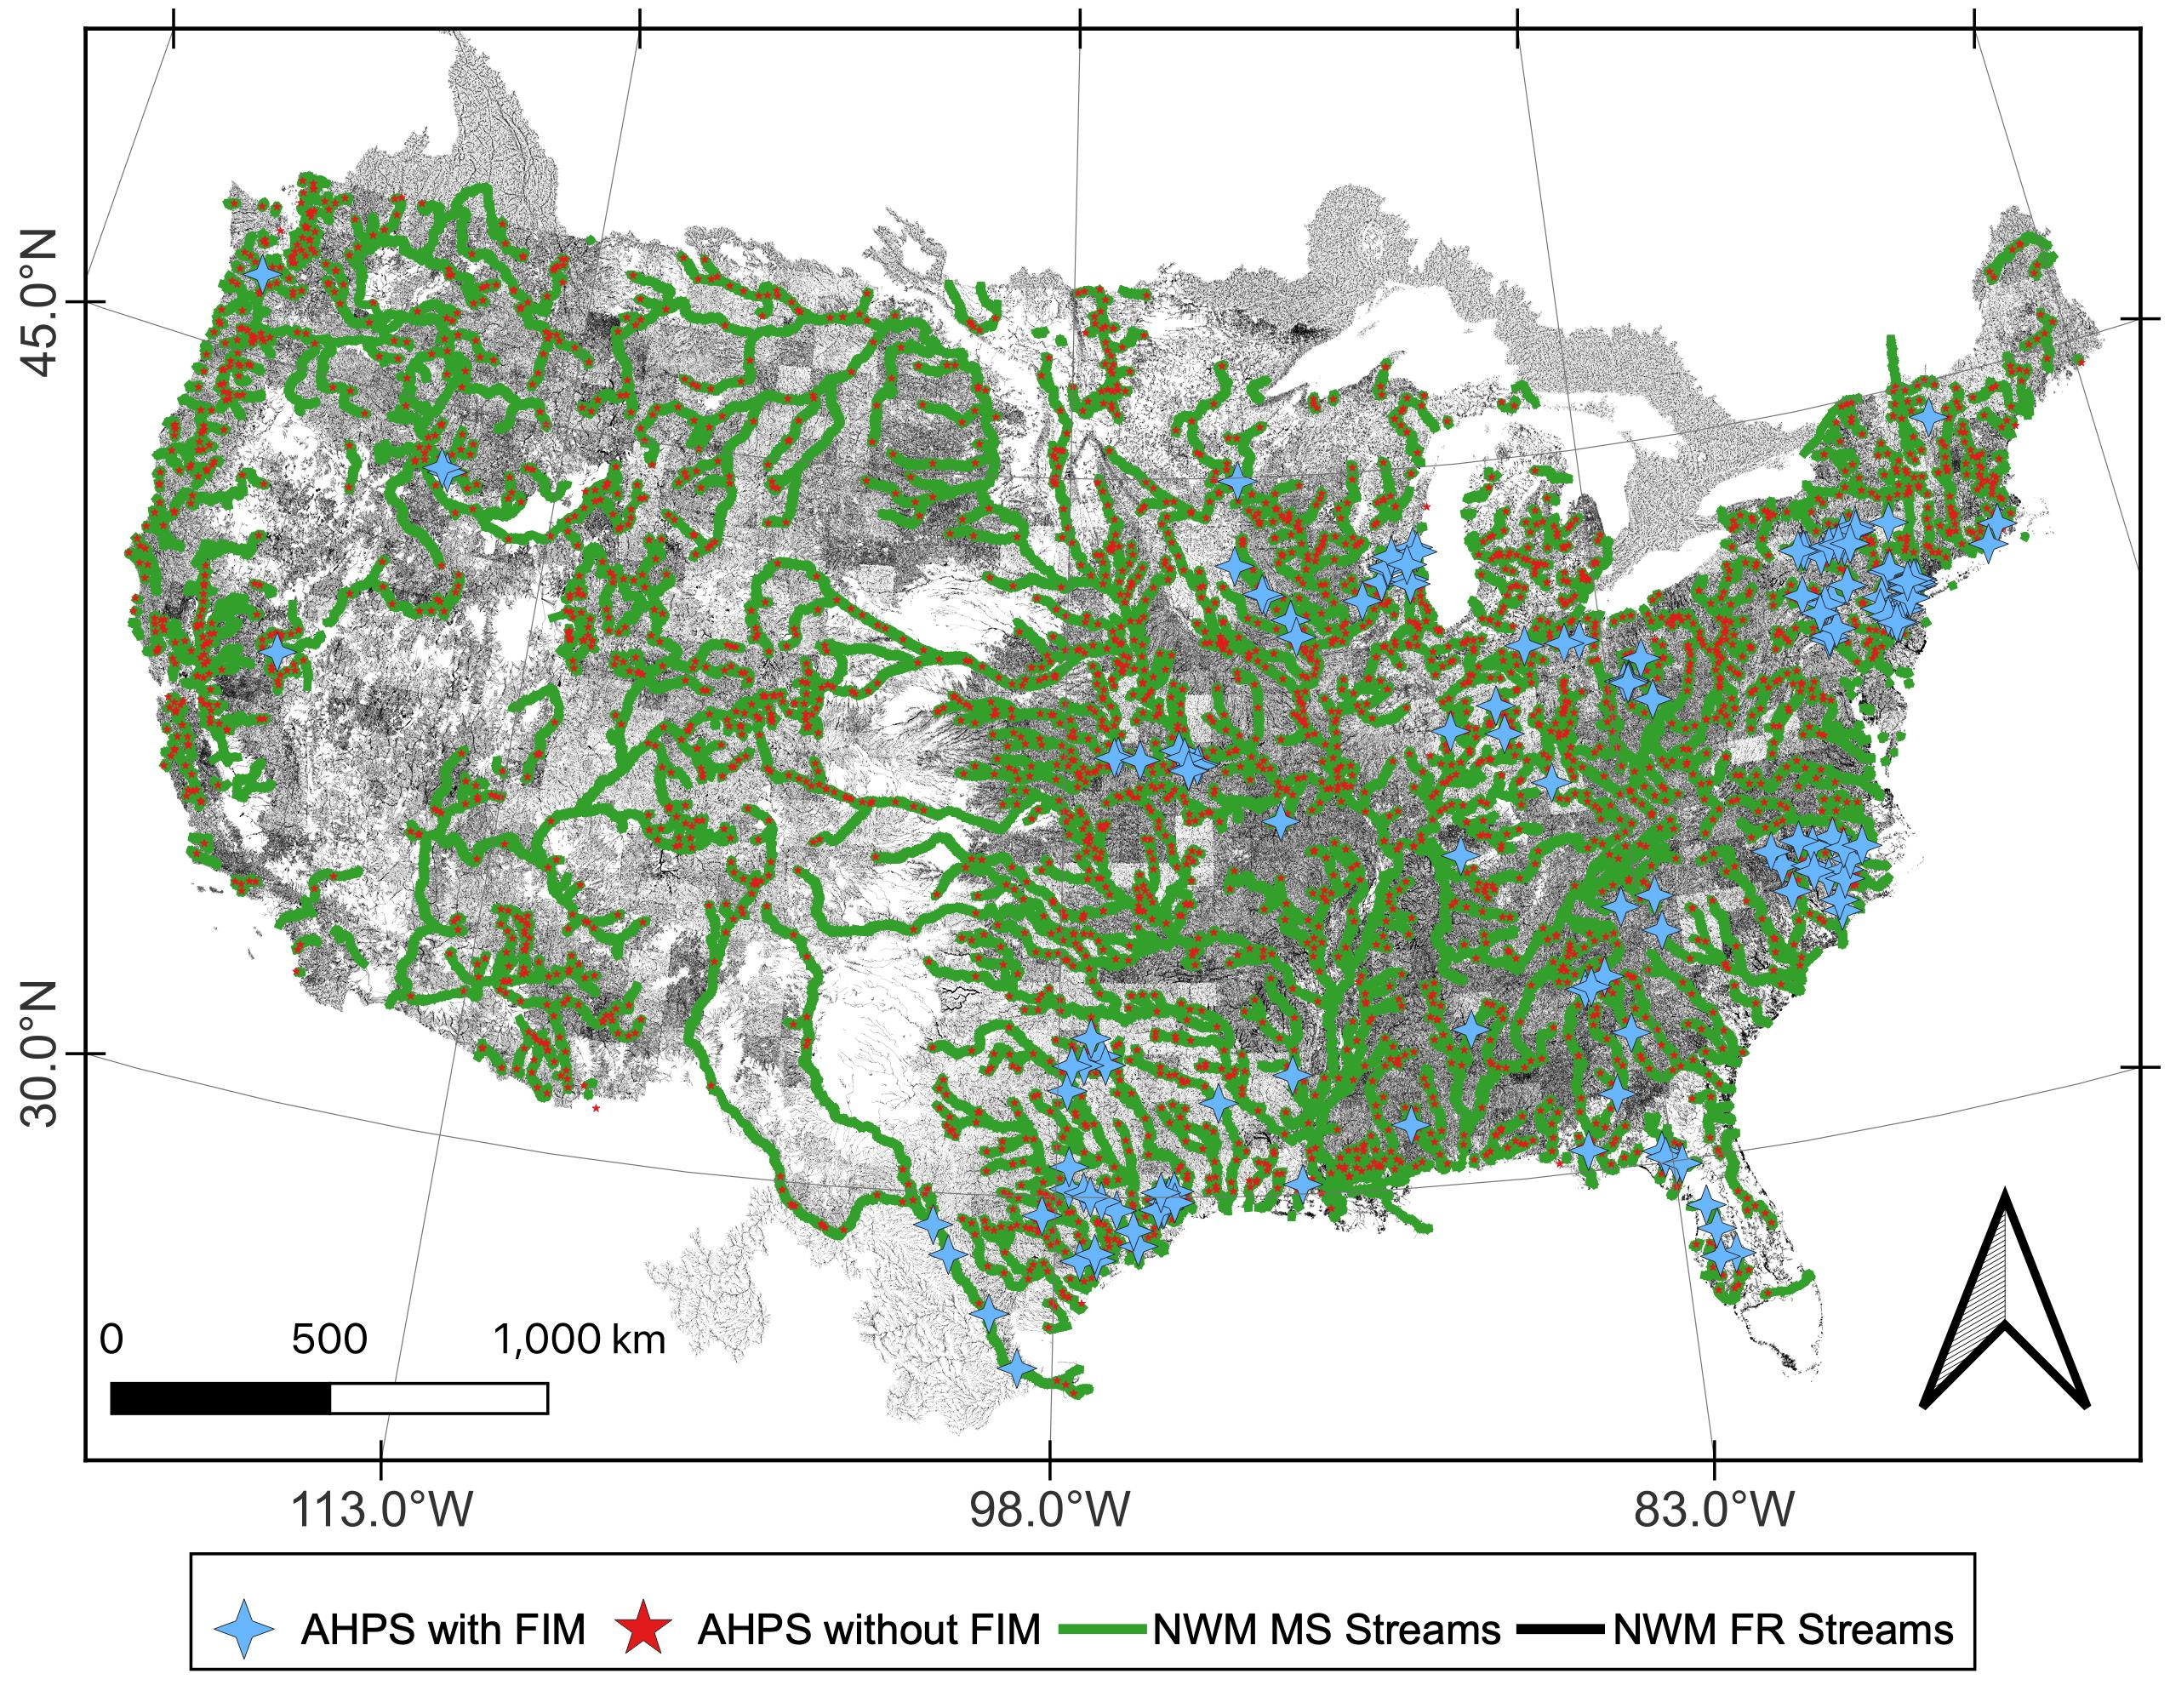
\includegraphics[scale=1.0]{figures/forecast_points.jpg}
\caption{Forecast points with and without FIM in United States' Advanced Hydrologic Prediction System.
Also show are the National Water Model stream networks at the full resolution (FR) and Mainstems (MS) resolution.}
\label{fig:forecast_points}
\end{figure}
%
%%%%%%%%%%%%%%%%%%%%%%%%%%%%%%%%%%%%%%%%%%%%%%%%%%%%%%%%
\subsection{National Water Model}
\label{ssec:national_water_model}
%%%%%%%%%%%%%%%%%%%%%%%%%%%%%%%%%%%%%%%%%%%%%%%%%%%%%%%%
%
Additional work is required to fill-in the gaps that the AHPS leaves in terms of spatial and temporal coverage.
In response to growing stakeholder demand for enhanced and integrated water resource forecasts, the Office of Water Prediction (OWP) at the National Water Center (NWC) along with its partners has developed and implemented operationally the National Water Model (NWM) which is a version of the Weather Research and Forecast Hydrologic Model (WRF-Hydro) \cite{gochis2018wrf,cosgrove2019evolution}. 
The NWM forecasts river discharges at more than 2.7 million forecast points at a variety of time horizons including some medium (10 day) and long (30 day) range forecast horizons.
The NWM enhances the spatial and temporal domain of the current AHPS capabilities operated at the 13 River Forecast Centers (RFC) in areas known as `hydro-blind'.
As a complement to the operational NWM, OWP has also developed a configuration of the NWM that extends RFC forecasts downstream by assimilating and routing forecast streamflows to the next downstream AHPS forecast point.
This configuration of the NWM is used to enhance forecasting skill by leveraging best available regional-scale data.
The river network upon which this special configuration operates is herein referred to as the Main-Stem (MS) modeling stream network.
Figure \ref{ssec:national_water_model} shows the Full-Resolution (FR) modeling stream network as well as the MS network.
The MS network contains roughly 120 thousand forecasting points or roughly 4.4\% of the reaches of the FR stream network.

The National Hydrography Dataset Plus (NHDPlus) V2.1 is the basis for the hydrofabric in the NWM due to its comprehensive use with the hydrologic communities' stakeholders \cite{mckay2012nhdplus}. 
The term hydrofabric is used within the NWM jargon to describe the subset of hydrography composed of the geospatial datasets required for hydrologic modeling including but not limited to stream networks, catchments, channel properties, and elevation data. 
The Muskingam-Cunge routing method is used within the NWM to reduce computational requirements of a continental scale model \cite{bedient2008hydrology,ponce1994variable,gochis2018wrf}.
Muskingam-Cunge routing scheme has been demonstrated by \citeA{cunge1969subject} to be equivalent to the convective-diffusive wave method without consideration to wave dampening.
As a result of high computational costs and large spatial domains, the need for high-resolution FIM at 10 m or better requires additional post-processing from the principal output of the NWM which is forecast river discharges at the reach scale. The Height Above Nearest Drainage (HAND) terrain model is one such technique that can be used, along with synthetic rating curves (SRC), to convert riverine discharges to stages then finally to inundation extents.
%
%%%%%%%%%%%%%%%%%%%%%%%%%%%%%%%%%%%%%%%%%%%%%%%%%%%%%%%%
\subsection{Height Above Nearest Drainage}
%%%%%%%%%%%%%%%%%%%%%%%%%%%%%%%%%%%%%%%%%%%%%%%%%%%%%%%%
%
HAND normalizes topography along the nearest drainage path and its been demonstrated to be a good proxy and indicator of a series of important environmental conditions including soil environments, landscape classes, soil gravitational potentials, geomorphologies, soil moisture, and groundwater dynamics \cite{renno2008hand,nobre2011height}. 
\citeA{nobre2016hand} showed evidence for utilizing the drainage normalizing HAND dataset as a proxy for flood potential to make static flood inundation maps from known stages.
A core assumption made for HAND based FIM is enforcing drainage across the entire area of interest which requires significant digital elevation maps (DEM) manipulations to make a reality.
The terrain index has even gone on to provide additional utility in the observation of riverine flood inundation mapping from remote sensing especially in areas of high electromagnetic interference such as vegetated and anthropogenic areas \cite{aristizabal2020high,shastry2019using,huang2017comparison,twele2016sentinel}.
\citeA{zheng2018river} developed a methodology for determining stage-discharge relationships known as synthetic rating curves (SRC) by sampling reach-averaged parameters from HAND datasets and inputting into the Manning's equation \cite{gauckler1867etudes,manning1890flow}.
This collection of methods, coupling HAND with SRCs, have been experimented with and compared to other sources of FIM including engineering scale models, in-situ observation, and remote sensing based observation with solid results in large spatial scale applications \cite{godbout2019error,johnson2019integrated,garousi2019terrain,nobre2016hand,afshari2018comparison,zheng2018geoflood,teng2015rapid,teng2017flood,zhang2018comparative}.
%
%%%%%%%%%%%%%%%%%%%%%%%%%%%%%%%%%%%%%%%%%%%%%%%%%%%%%%%%
\subsection{HAND Implementations}
%%%%%%%%%%%%%%%%%%%%%%%%%%%%%%%%%%%%%%%%%%%%%%%%%%%%%%%%
%
Due to significant advances in high-performance computing (HPC) and large scale high-resolution DEMs such as the 3D Elevation Program (3DEP) seamless at the 1/3 arc-second (10 m) scale, HAND has been implemented into software for large-scale, continental computation. 
As part of the OWP's Innovators Program and NWC's Summer Institute, the National Flood Interoperability Experiment (NFIE) generated FIM hydrofabric (will be used interchangeably with the datasets produced by HAND) rapidly on a high-performance computer (HPC) \cite{maidment2017conceptual,liu2016cybergis}. 
NFIE used open-source dependencies including the Terrain Analysis Using Digital Elevation Models (TauDEM) \cite{tarboton2005terrain} and the Geospatial Data Abstraction Library (GDAL) \cite{warmerdam2008geospatial} to compute HAND for the Continental United States (CONUS) at 331 Hydrologic Unit Code (HUC) 6 processing units in 1.34 CPU years.
By allocating 31 nodes at 20 cores per for a total of 620 available cores to the overall operation, it enabled the production to finish up in 36 hours consuming 3.2TB of peak memory and 5TB of total disk space.
Originally, NFIE utilized the NHD Medium Resolution (MR) to etch or burn flowlines prior to further conditioning but more recent work has advanced this to the more current NHDPlus High Resolution (HR) \cite{liu2020height}. 
The original NFIE dataset was employed by the NWC as an unofficial demonstrations to produce forecast FIM from the NWM for additional guidance in hydro-blind regions.
Further work by \citeA{djokic2019arc}, implemented a series of improvements to HAND including equidistant reaches, updates to use with NHDPlusHR hydrography, and AGREE-DEM reconditioning \cite{hellweger1997agree} into an ESRI Arc-Hydro workflow with use in ArcGIS. 
More notably the software added the ability to derive drainage potentials on both the NWM FR and MS stream networks which leverages the lower drainage density and Horton-Strahler stream order of the MS network.

Related to these efforts, the USGS has invested in relative elevation HAND-like methods via work in the GIS Flood Tool (GFT) that also uses synthetic rating curves with cross-sections for stage-discharge relationships \cite{verdin2016software}.
Additional investment by \citeA{petrochenkov2020pygft} was able to successfully scale this approach by transitioning the method to open-source Python source code (PyGFT) and implementing novel interpolation methods to help address some of the catchment boundary discontinuities discussed more in this paper.
In addition to the domestic work done in the US, some studies have expanded upon HAND to cover global domains at 30 m resolutions \cite{yamazaki2019merit,donchyts2016global}.
%
%%%%%%%%%%%%%%%%%%%%%%%%%%%%%%%%%%%%%%%%%%%%%%%%%%%%%%%%
\subsection{OWP FIM}
%%%%%%%%%%%%%%%%%%%%%%%%%%%%%%%%%%%%%%%%%%%%%%%%%%%%%%%%
%
Many of those in the academic community assessing HAND's efficacy for producing FIM have noted opportunities for improvement. 
\citeA{godbout2019error} found how reach length and slope are important parameters for maximizing mapping skill with the moderate values performing best. 
The co-linearity of reach length and slope led \citeA{godbout2019error} to propose that reaches of extreme lengths performed worse because of the extreme slope values, a parameter directly represented in Manning's equation. 
Issues with the reach-average approaches have been documented in \citeA{tuozzolo2019impact} where large within reach variance of the roughness Manning's n coefficient have been observed.
Furthermore, \citeA{garousi2019terrain} noted improvements to mapping efficacy by conditioning monotonically decreasing thalweg elevations, adjusting the Manning's n roughness coefficient, and using higher resolution (3 m) Digital Elevation Model's (DEM) derived from light detection and ranging (Lidar).
The use of higher resolution DEMs in that study was motivated by previous work with Lidar DEMs and least-cost thalweg derivations \cite{zheng2018geoflood}.
Further work by \citeA{johnson2019integrated} noted the general under-prediction of HAND and suggested tuning the Manning's n parameter to better align SRC's with observations. 
Additionally, the sensitivity to low topographic relief and channel slope have been observed \cite{johnson2019integrated,godbout2019error}. 
Most notably, HAND has been shown to demonstrate sensitivity to drainage network density known colloquially as the catchment boundary problem \cite{zhang2018comparative,mcgehee2016modified,li2020evaluation,nobre2016hand}.
This sensitivity is noted at higher order streams with large flows and low Froude numbers and is manifested by a constriction in the inundation extents at the junction location.
These findings suggest improvements to HAND are required that utilize advanced computational algorithms and software to compute a FIM hydrofabric required for producing continental-scale FIM.

With all of the latest developments in the realm of continental FIM (CFIM) noted in the previous paragraph, a fast, open-source framework for accelerating the research to operations pipeline is required.
Here we introduce OWP FIM that utilizes a few of the latest techniques in HAND based FIM oriented for use with the NWM in continental scale operational forecasting settings. 
This framework is open-source and modular enabling and accelerating the research to operations development pipeline.
Automated evaluation tools and processed test case data enable the rapid testing and evaluation of new techniques in consistent contexts.
In addition to developed tooling, we introduce research demonstrating how FIM performance skill with HAND can be improved by reducing Horton-Strahler stream orders \cite{horton1945erosional,strahler1952hypsometric,strahler1952hypsometric} of the stream networks.
Previous authors dating back to the first HAND for FIM work by \citeA{nobre2016hand} have noted a sensitivity of mapping skill to stream threshold which serves as a proxy for stream density and the maximum Horton-Strahler stream order (or simply stream order) of the processing unit employed \cite{zhang2018comparative,mcgehee2016modified,li2020evaluation}.
Here we demonstrate how reducing a HAND processing unit's stream network to a singular stream order discretized by level paths, can enhance FIM skill.
This capability will be referred to as Generalized Mainstems (GMS).
The following methods and results describe the work in more detail and demonstrate its efficacy in producing enhanced FIM for the NWM with applications.
%
 %
% Materials and Methods
\clearpage % this clears figures before references
%%%%%%%%%%%%%%%%%%%%%%%%%%%%%%%%%%%%%%%%%%%%%%%%%%%%%%%%

%%%%%%%%%%%%%%%%%%%%%%%%%%%%%%%%%%%%%%%%%%%%%%%%%%%%%%%%
\section{Materials and Methods}
%%%%%%%%%%%%%%%%%%%%%%%%%%%%%%%%%%%%%%%%%%%%%%%%%%%%%%%%
%%%%%%%%%%%%%%%%%%%%%%%%%%%%%%%%%%%%%%%%%%%%%%%%%%%%%%%%
%
OWP FIM is a fully operational pipeline of software tools to help acquire datasets, cache hydrofabrics, produce FIMs, and evaluate results.
%
%%%%%%%%%%%%%%%%%%%%%%%%%%%%%%%%%%%%%%%%%%%%%%%%%%%%%%%%
\subsection{Software Dependencies and Architecture}
%%%%%%%%%%%%%%%%%%%%%%%%%%%%%%%%%%%%%%%%%%%%%%%%%%%%%%%%
%
OWP FIM exclusively utilizes free and open source software dependencies including Python 3, GDAL, TauDEM, Geographic Resource Analysis Support System (GRASS), GNU Parallel, and MPICH \cite{python382,gdal2020,tarboton2005terrain,grass2020,tange2015gnu,amer2021mpich}.
Within the Python 3 ecosystem, many common packages are employed including but not limited to RichDEM, GeoPandas, Rasterio, Rasterstats, and Numba \cite{barnes2018richdem,jordahl2014geopandas,lam2015numba}. 
To simplify setup and enhance portability across host operating systems OWP FIM packages all dependencies up in a Docker image (\url{https://docs.docker.com/engine/install/}). 
A user only needs to install Docker on their host machine and build the image from the provided recipe. 
Source code is made available for this project on GitHub \cite{inundationMapping2022}. 

The pipeline is discretized into key areas that a user can interact with to reproduce the results of this study. 
Preprocessing acquires and prepares datasets for production of the FIM hydrofabric. 
The FIM hydrofabric is defined as the datasets required to make an inundation map from discharges including the relative elevation model (REM) or HAND grid, the catchments in vector and raster form, and the hydro-table (contains synthetic rating curves and cross-walk information).
Functionality is included to turn FIM hydrofabric and streamflows into inundation maps represented in both binary and depths.
Lastly, a test suite includes means of calculating evaluation metrics compared to a variety of preprocessed test case data.
A user should visit the Readme.md page on GitHub for more information on how to acquire the datasets and reproduce the pipeline.
%
%%%%%%%%%%%%%%%%%%%%%%%%%%%%%%%%%%%%%%%%%%%%%%%%%%%%%%%%
\subsection{Datasets}
\label{ssec:datasets}
%%%%%%%%%%%%%%%%%%%%%%%%%%%%%%%%%%%%%%%%%%%%%%%%%%%%%%%%
%
Data sources used within OWP FIM are publicly available from a variety of government sources including the USGS, NWC, Federal Emergency Management Agency (FEMA), and US Army Core of Engineers (USACE) to enhance reproducibility and collaboration among government, academia, and industry.
Instructions for accessing data are provided on the project's GitHub page via an Amazon Web Services (AWS) S3 bucket furnished by Earth Science Information Partners (ESIP) \cite{esipData2022}.
The National Hydrography Dataset Plus High Resolution (NHDPlusHR) Beta Version is the latest hydrography dataset used for land surface hydrologic modeling in the US \cite{moore2019user}. 
It is used in conjunction with the hydrofabric of the NWM V2.1 to help define flowlines for OWP FIM while the NWM hydrofabric is also used to define reservoirs for exclusion and catchments to cross-walk to for forecasting purposes.
For enforcing levee data into the DEMs, the USACE National Levee Database (NLD) is used to burn feature elevations \cite{engineers2016national}.
Since NHDPlusHR datasets extend beyond land borders into sea and Great Lake regions, we used the land-sea border from OpenStreetMap (OSM) and the land-lake border from Great Lakes Hydrography Dataset (GLHD) to exclude those areas from production of FIMs \cite{OpenStreetMap,GreatLakesHydrographyDataset}.
Additionally, the Base Level Engineering (BLE) datasets within FEMA Region 6 spanning parts of 9 states including Colorado, New Mexico, Texas, Oklahoma, Kansas, Arkansas, Louisiana, Missouri and Mississippi at two recurrence intervals, 1\% (100 year) and 0.2\% (500 year), are used as validation in this study and furnished by the Interagency Flood Risk Management (InFRM) consortium \cite{fema2021base,fema2021estimated}. 
These BLE datasets are provided at the watershed scale (HUC8) utilizing best available simulations and DEMs.
The full input datasets presented by source are listed in Table \ref{tab:data}.
%
\begin{table}
\caption{Data sources, names, and descriptions.}
\label{tab:data}
\centering
\begin{tabular}{|p{2cm}|p{4cm}|p{8cm}|}
%\begin{tabular}{l c c}
\hline
Source & Name & Description \\
\hline
USGS & NHDPlusHR BurnLineEvents & Stream lines used by NHDPlus HR for hydro-enforcement \\
\hline
USGS & NHDPlusHR Value-Added Attributes & Database of additional attributes associated with the BurnLineEvents that enhance navigation, analysis, and display \\
\hline
USGS & NHDPlusHR DEM & DEM used for NHDPlus HR at 1/3 arc-second (10 m) spatial resolution and vertical units in centimeters \\
\hline
NOAA-OWP & NWM Streams & Stream network center lines used by NWM for routing and forecasting. \\
\hline
NOAA-OWP & NWM Catchments & Surface drainage area corresponding to each reach in the NWM. \\
\hline
NOAA-OWP & NWM Waterbodies & Waterbodies considered by the NWM as reservoirs or lakes. \\
\hline
USACE & NLD & Levee database of locations and elevations  \\
\hline
OSM & Land-Sea Border & Border of land and sea. \\
\hline
GLHD & Land-Great Lakes Border & Border of land and Great Lakes. \\
\hline
InFRM & Cross-Sections & HEC-RAS 1-D cross-sections used for modeling in BLE datasets. Includes discharges for 1\% and 0.2\% recurrence interval events. \\
\hline
InFRM & Flood Inundation Extents & Inundation depths produced by InFRM BLE HEC-RAS 1D for 1\% and 0.2\% recurrence interval events. \\
\hline
\end{tabular}
\end{table}
%
Areas with all the required data (from the NWM and the USGS) are labeled as the FIM domain which includes 2,188 HUC8s for the FR and GMS networks and 1,604 HUC8s for the MS method. 
These methods will be explained more later.
An enhancement of OWP FIM over previous HAND based FIM versions is the support for Hawaii and Puerto Rico which the NWM V2.1 will cover.
%
%%%%%%%%%%%%%%%%%%%%%%%%%%%%%%%%%%%%%%%%%%%%%%%%%%%%%%%%
\subsection{Hydro-conditioning}
\label{ssec:hydro_conditioning}
%%%%%%%%%%%%%%%%%%%%%%%%%%%%%%%%%%%%%%%%%%%%%%%%%%%%%%%%
%
The DEM is subject to a series of hydro-conditioning procedures to enhance its suitability for riverine flood inundation mapping. 
These techniques are specific for making OWP FIM and differ from the conditioning methods used by the NHDPlusHR Beta \cite{moore2019user}.
HAND inherently requires all areas eligible for inundation to drain to the designated drainage network so DEMs must undergo significant manipulation to make this the case.
In other words, all areas within a given processing unit for HAND must have monotonically decreasing elevations if we wish to have them be eligble for flooding.
Hydro-conditioning is implemented to obtain many objectives including enforcing the location of hydrologically relevant features such as flowlines, lakes, or drainage divides whether natural or anthropogenic. 
It can also be used to simulate more accurate bathymetry which is not accounted for in the 10 m DEM \cite{gesch2002national}.

Specifically within the context of OWP FIM, the hydro-conditioning operations that take place in sequential order are presented. 
Prior to any hydro-conditioning, all input datasets must be subset from their original spatial domain scales into the processing units of size HUC8. 
The subsetting is done by spatial query for the cases of the levees, DEM, and NWM hydrofabric while the NHDPlusHR BurnLineEvents are subset via attribute query for the given reach code's membership in the processing unit.
Hydro-conditioning raster operations take place on buffered boundary definitions to avoid edge contamination and effects \cite{lindsay2013measuring}. 
%
%%%%%%%%%%%%%%%%%%%%%%%%%%%%%%%%%%%%%%%%%%%%%%%%%%%%%%%%
\subsubsection{Stream Network Enforcement} 
\label{ssec:stream_network_enforcment}
%
The location of the stream network is enforced to ensure general agreement with established stream networks.
The NHDPlusHR Beta Burnline Event layer is used to enforce stream locations in the NHDPlusHR workflow so it is also used here for hydro-enforcement \cite{moore2019user}. 
However, to better match the drainage density of the NWM V2.1 stream network which is based on the NHDPlus Medium Resolution, the Burnline Events are pruned utilizing a nearest neighbor search around the NWM flowlines.
For every NWM headwater segment a headwater point is derived and linearly interpolated to the nearest Burnline Event segment.
Burnline Event headwater segments are split at the adjusted headwater point to match NWM flowlines.
The resulting pruned NHD stream network is what gets hydro-enforced in subsequent operations.
This procedure is best illustrated in Figure \ref{fig:stream_density_pruning} which shows that the pruned NHD network corresponds to the full density NHD network at NWM V2.1 headwater locations only. 
Additionally, the NHDPlusHR pruned headwaters are later used for seeding a new FIM drainage network that best agrees with the DEM after all hydro-conditioning takes place.
%
\begin{figure}[h!]
\centering
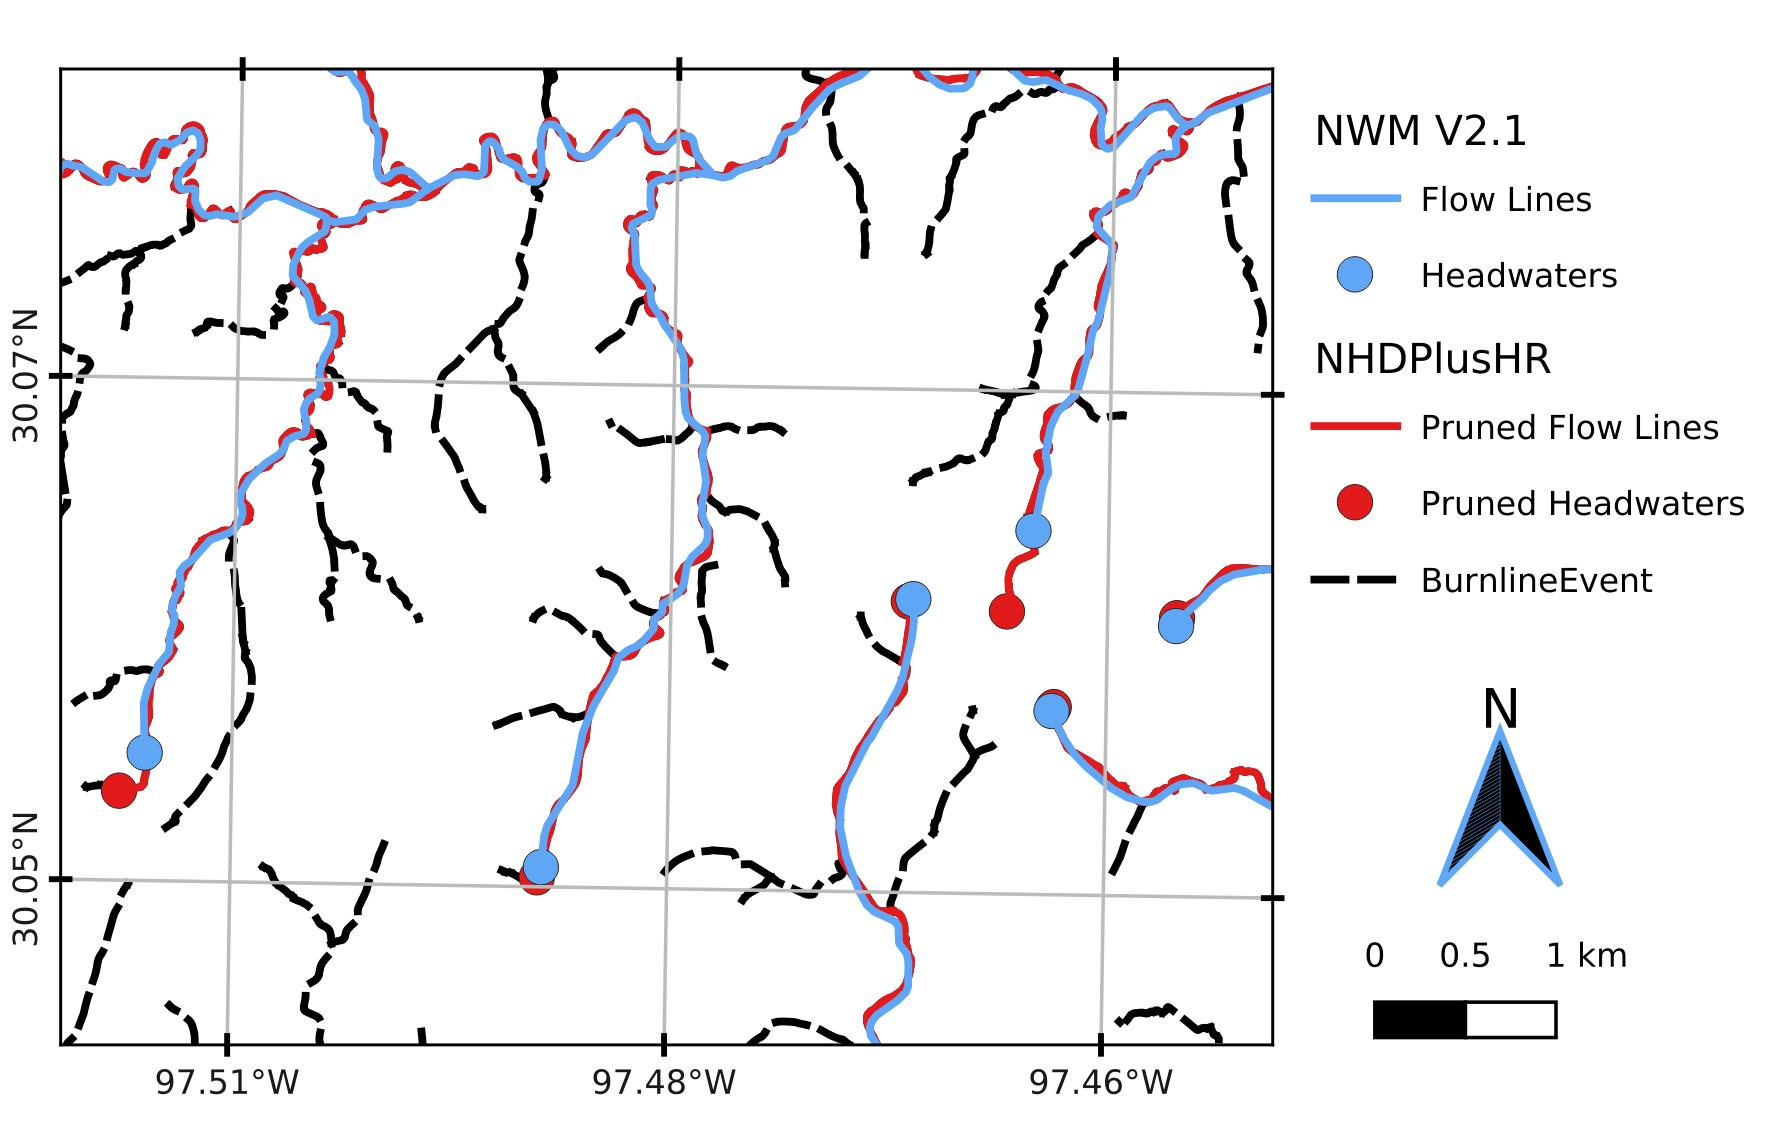
\includegraphics[scale=1.0]{figures/headwaters.jpg}
\caption{Pruning of NHDPlus HR Beta Burnline Events (dotted black) to NWM V2.1 stream density (blue) using nearest neighbor selection and linear interpolation. Resulting stream network (red) matches the drainage density of NWM V2.1 while corresponding spatially with the NHDPlusHR Burnline Events.}
\label{fig:stream_density_pruning}
\end{figure}
%
This results in a stream network that has the same density as the NWM V2.1 flowline network but utilizes the locations of the NHDPlusHR Beta BurnLineEvents. 

The pruned stream network is then utilized to hydro-enforce the DEM with a methodology developed by \citeA{hellweger1997agree} known as the AGREE DEM Surface Reconditioning System. 
The AGREE algorithm seeks to burn artificially deep thalweg elevations by a uniform value known as sharp drop. 
The modification continues by excavating an area of a given buffer distance from the thalweg by a depth proportional to the distance from the channel given by the smooth drop. 
The resulting enforcement of the thalweg and general bathymetric region results in a cross-section resembling a trapezoidal shape with a significantly lower elevation along the thalweg line only.
In total, the AGREE algorithm requires three parameters including the buffer distance, smooth drop, and sharp drop. 
Using the AGREE method as opposed to simple thalweg burning techniques helps prevent distortions in the delineation of streams as well as the catchment boundaries \cite{saunders1995grid,saunders1996gis,mizgalewicz1996modeling,hellweger1997agree,quenzer1998gis,baker2006comparison}.
\citeA{baker2006comparison} noted AGREE produced satisfactory results when compared to other enforcement especially when computational costs are considered. 
Downsides to the technique include the possibility of exhibiting parallel streams where the burned stream and real stream are both represented \cite{hellweger1997agree,saunders1999preparation} and some distortion of the catchment boundaries can also be observed \cite{saunders1999preparation,saunders1996gis}. Some of these drawbacks are later addressed by additional conditioning techniques later on.
%
%%%%%%%%%%%%%%%%%%%%%%%%%%%%%%%%%%%%%%%%%%%%%%%%%%%%%%%%
\subsubsection{Levee Enforcement}
%
The DEM at 10 m resolution lacks sufficient representation of fine grain features such as embankments, floodwalls, and closure structures.
In order to better represent the influences of these features upon hydraulics and inundation extents, the National Levee Database (NLD) published by USACE was used to enforce elevations within the 10 m DEM.
The elevations found in the NLD are burned into the DEM if those elevations were found to exceed those already in place.
%
%%%%%%%%%%%%%%%%%%%%%%%%%%%%%%%%%%%%%%%%%%%%%%%%%%%%%%%%
\subsubsection{Depression Filling}
\label{sssec:depression_filling}
%
Local depressions are naturally occurring features of a DEM but must be addressed if a connected drainage network with continuous catchments are to be derived for flood modeling purposes.
The conditioned DEM was removed of depressions by filling areas with pits while preserving the stream and levee information previously enforced.
Priority-Flood developed by \citeA{barnes2014priority} is an algorithm for filling said depressions and shown to have improved performance over early works in the field by \citeA{jenson1988extracting} implemented in \citeA{tarboton2005terrain} as well as \citeA{planchon2002fast}.
The depression filling algorithm used in our pipeline is a Priority-Flood variant developed by \cite{zhou2016efficient} with enhanced single-thread performance and a time complexity of O(n log n) for floating point grids.
This performance was enabled by limiting the processing queue with a region-growing method to exclude many of the slope cells \cite{zhou2016efficient}.
The depression technique employed here does leave the existence of flat regions where pits existed a prior thus later requiring the need for resolving these flats.
The enhanced variant of Priority-Flood is implemented and made available by \citeA{barnes2018richdem} and \citeA{zhou2015filldem}.
%
%%%%%%%%%%%%%%%%%%%%%%%%%%%%%%%%%%%%%%%%%%%%%%%%%%%%%%%%
\subsubsection{Stream Thalweg Elevation Conditioning}
\label{sssec:stream_thalweg_elevation_conditioning}
%
Thalweg elevations are critical components of relative elevation based inundation mapping thus much is performed to ensure the best available, monotonically decreasing elevations are derived prior to normalizing of elevations.
In order to prevent situations where the burned thalweg and the thalweg endemic to the DEM run parallel to one another, the normalized excavation algorithm \cite{saunders1999preparation} is used to seek a zonal (nearest neighbor) elevation minimum for each thalweg pixel. 
Each zone is defined as the thalweg's pixel nearest neighborhood within a maximum distance of 50 m.
The zonal minimum is computed for each thalweg pixel zone and the minimum is used to replace the existing thalweg elevation value.

The next step involves conditioning these local minimums along the thalweg to enforce monotonically decreasing thalweg elevations for FIM.
\citeA{garousi2019terrain} proposed an algorithm that traverses stream thalweg pixels in a depth first manner starting with adding all the headwater pixels to a queue. 
The connectivity of the thalweg pixels is defined by the D-8 flow directions further discussed in Section \ref{ssec:flow_direction_and_flat_resolution}.
At every thalweg pixel, the minimum elevation among itself and its upstream contributing thalweg pixels is taken as shown in Equation \ref{eq:thalweg_breach},
%
\begin{linenomath*}
\begin{equation}
\label{eq:thalweg_breach}
\textbf{D}[x] = \min_{y\ drains\ to\ x} {(\ \textbf{D}[x]\ ,\ \textbf{D}[y]\ )}
\end{equation}
\end{linenomath*}
%
, in which \textbf{D} represents the array of thalweg adjusted elevations indexed by x and y where by y is upstream of x. 
When a pixel's upstream neighbors are all evaluated, the downstream pixel is added into the queue thus the depth first traversal of the drainage network.
This procedure enforces the location of streams and ensures that thalweg elevations are hydrologically correct which yielded a 7\% improvement in Critical Success Index (CSI) per an evaluation for an event in 2017 on the Malad river \cite{garousi2019terrain}.
%
%%%%%%%%%%%%%%%%%%%%%%%%%%%%%%%%%%%%%%%%%%%%%%%%%%%%%%%%
\subsection{Deriving FIM Hydrofabric}
\label{ssec:deriving_fim_hydrofabric}
%%%%%%%%%%%%%%%%%%%%%%%%%%%%%%%%%%%%%%%%%%%%%%%%%%%%%%%%
%
The FIM Hydrofabric is defined here as the collection of geospatial datasets that are used for converting NWM discharges into inundation extents.
%
%%%%%%%%%%%%%%%%%%%%%%%%%%%%%%%%%%%%%%%%%%%%%%%%%%%%%%%%
\subsubsection{Flow Directions and Flats Resolution}
\label{ssec:flow_direction_and_flat_resolution}
%
To facilitate the generation of a connected stream network and its associated catchments from the conditioned DEM, the depression-filled DEM is used to derive connectivity in the form of D-8 flow directions.
D-8 seeks to allocate a drainage direction for every pixel based on the adjacent eight pixel neighborhood with the steepest slope \cite{o1984extraction}.
The horizontal component of slope is defined as one for the 4 neighboring pixels in the main cardinal directions while the intercardinal pixels are designated a horizontal component of $\sqrt{2}$. 
The flow direction is encoded as integers 1 through 8 corresponding with the cardinal direction East as 1 and continuing counter-clockwise to the Southeast direction as 8. 
Flow directions are derived for non-depression filled regions trivially with the above procedure but to define connectivity for every grid cell the remaining flats corresponding to depression filled cells must be resolved.

Flat resolution from flats endemic to the DEM or from depression filled regions is a costly, non-trivial procedure which was originally addressed by \citeA{garbrecht1997assignment}.  
Software implementations have developed means to partition the problem and resolve flats iteratively with communication across processes \cite{tarboton2009generalized,tesfa2011extraction,wallis2009parallel,tarboton2005terrain}.
The excessive iteration and communication leads to poor computational performance which motivated further work on how to optimize flat resolution \cite{survila2016scalable,barnes2014efficient}.
Specifically the work by \citeA{survila2016scalable} enables the use of parallel processing and made smoother catchments from our informal experience than those from \citeA{barnes2014efficient}.
By processing flats local to each partition separately from flats shared with other partitions, the accelerated flat resolution algorithm demonstrated an average speed up of 468x when compared to prior implementations \cite{survila2016scalable}.
OWP FIM utilized a CyberGIS implementation of the D-8 flow direction algorithm with the accelerated resolution of flats \cite{survila2016scalable,cybergis2016}.
%
%%%%%%%%%%%%%%%%%%%%%%%%%%%%%%%%%%%%%%%%%%%%%%%%%%%%%%%%
\subsubsection{Deriving FIM Stream Network}
\label{sssec:deriving_fim_stream_network}
%
The derivations of relative elevations and catchments from the newly conditioned DEM involves re-deriving a new FIM stream network. 
The FIM stream network is of similar drainage density as the NWM V2.1 network but fully converges at all junctions leaving no divergences in the network.
This is accomplished by using the seed points generated from the stream network enforcement process (Section \ref{ssec:stream_network_enforcment}).
These seeds points are headwater locations of the NHDPlusHR Beta Burnline Events layer that spatially correspond to the headwater definitions in the stream network of the NWM V2.1.
Feeding the seed points and previously computed flow directions into flow accumulation methods \cite{wallis2009parallel,tarboton1997new,tarboton2005terrain} yields a stream link accumulation raster that can be converted to a vector file for further processing.
Each stream link in this derived FIM stream network is split into equidistant reaches.
Stream links are defined here as segments of rivers discretized by junctions with other NWM river segments.
Stream links are then further segmented at NWM lakes and HUC8 boundaries.
Discretizing at NWM lakes isolates reaches and catchments associated with lakes and reservoirs to avoid mapping them using the Manning's equation and could potentially enable volume based mapping in the future as a feature enhancement.
Based on previous research, splitting each remaining stream link into equidistant reaches not to exceed a parameterized value of 1.5 km helps improve synthetic rating curve and mapping skill \cite{garousi2019terrain,godbout2019error,zheng2018geoflood}.
Small reaches can lead to unrealistic variances in channel geometries while oversized reaches can lead to grouping too much slope variance into one discretation of the stream network.
Short stream segments that are introduced as a result of forced network breaks due to reservoir, levee, or HUC boundaries inherent the synthetic rating curve properties of the upstream or downstream segment, depending on the topology.
Section \ref{sssec:synthetic_rating_curve} details the derivation of the synthetic rating curves and the dependence on channel length. 
Additionally every reach (and later catchment) is assigned a globally unique identifier based on the HUC 8 membership.
This stream network is important since it drives the HAND calculation and derivation of catchments.
%
%%%%%%%%%%%%%%%%%%%%%%%%%%%%%%%%%%%%%%%%%%%%%%%%%%%%%%%%
\subsubsection{Catchments}
\label{sssec:catchments}
%
Catchments were derived using the D8 connectivity established by \citeA{o1984extraction}.
Outlet points are set at the pixel center points of the delineated stream lines explained in Section \ref{sssec:deriving_fim_stream_network}.
The outlets act as root nodes in a tree structure and the connectivity is traversed to derive the contributing area for each gage.
Two sets of catchments are derived, one of which assigns the contributing area for each thalweg pixel which is used for relative elevation calculation.
The other catchments are derived for the contributing area for each stream reach as defined in Section \ref{sssec:deriving_fim_stream_network}. 
%
%%%%%%%%%%%%%%%%%%%%%%%%%%%%%%%%%%%%%%%%%%%%%%%%%%%%%%%%
\subsubsection{Height Above Nearest Drainage}
%
Once the pixel level catchments are derived, the final relative elevations can be computed.
Every non-thalweg elevation is subtracted from the thalweg elevation within the same pixel-level catchment described in Section \ref{sssec:catchments}.
The DEM used for this operation is the DEM resulting from the thalweg conditioning procedures described in Section \ref{sssec:stream_thalweg_elevation_conditioning}.
Outside of the excavated channel from the AGREE DEM method, the native non-drainage enforced elevations are used to reduce sources of error in relative elevations due to pit filling. 
%
%%%%%%%%%%%%%%%%%%%%%%%%%%%%%%%%%%%%%%%%%%%%%%%%%%%%%%%%
\subsubsection{Synthetic Rating Curves}
\label{sssec:synthetic_rating_curve}
%
 A method for converting forecast river discharges from the NWM to stages or river depths is necessary for producing FIMs with HAND. 
For one-dimensional models such as the NWM, the typical procedure is to establish the stage-discharge relationship by sampling data from the DEM to derive a synthetic rating curve at discrete cross-sections \cite{quintero2021development,di2011hydraulic}. 
For this application, we utilized the reach averaged approach for developing synthetic rating curves (SRC) \cite{zheng2018river}.
The reach averaged approach seeks to sample the geometry parameters in the Manning's equation \cite{gauckler1867etudes,manning1890flow} on a reach scale then dividing those by length. 
The reach averaged Manning's formula is derived to be 
%
\begin{linenomath*}
\begin{equation}
\label{eq:reach_averaged_mannings_equation}
\textbf{Q} = \frac{1}{n} \frac{V^{5/3}S^{1/2}}{L B^{2/3}} 
\end{equation}
\end{linenomath*}
%
where Q is discharge, y indicates the stage, n is the Manning's n roughness coefficient, V is volume at stage y, S is channel slope, L is along flow length, and B is wetted bed area at stage y.
Q, V, and B are taken a specific y values so are more formally written as $Q = Q(y)$, $V = V(y)$, and $B = B(y)$, respectively.
All units are international given the 1 numerator above n.
The reach averaged method has been compared to rating curves from Hydrologic Engineering Center\'s River Analysis System (HEC-RAS) and USGS gages yielding comparable results for estimating the river bottom elevation profile, channel width at given stages, and stage-discharge relationships \cite{zheng2018river}.
The reach averaged geometry parameters including number of wet cells, bed area, and volume are sampled from the thalweg conditioned AGREE DEM using TauDEM's catchhydrogeo utility.
Using the split reaches described in Section \ref{sssec:deriving_fim_stream_network}, the channel slope is sampled from the thalweg conditioned DEM at the end points of the reaches while the same reaches are used to calculate the channel length.


Setting of the Manning's n roughness coefficient has precedent in previous CFIM studies \cite{maidment2017conceptual,liu2016cybergis,liu2020height,djokic2019arc,garousi2019terrain,zheng2018geoflood} with two noted values of 0.05 and 0.06 for NFIE and \citeA{djokic2019arc} respectively. 
These values are applied universally to the entire forecasting domain across space, time, and discharge profiles.
We note significant opportunity to enhance CFIM skill by better parameterizing Manning's n according to available data including but limited to land cover, land use, stream order, stream geometry, drainage area, reach length, and discharge percentiles \cite{garousi2019terrain,johnson2019integrated}.
For now and for the purpose of this study, we examine the developed ecosystem of tools with Manning's n set to both 0.06 and 0.12 which we hope will shed some light on the sensitivity of this parameter to HAND based FIMs.
After all the parameters to the Manning's equation have been determined with either hydrofabric sampling or user parameterization, we select 84 stage values from 0 to 25 meters in depth at one third of a meter increments to calculate the discharge values for each stage value. 
%
%%%%%%%%%%%%%%%%%%%%%%%%%%%%%%%%%%%%%%%%%%%%%%%%%%%%%%%%
\subsubsection{Cross-walking with NWM Stream Network}
\label{sssec:cross_walking_networks}
%
The stream network derived in Section \ref{sssec:deriving_fim_stream_network} must be associated with a NWM reach identifier so that a discharge can be converted to stage and later inundation extent.
For the methods already discussed, we overlap the reach catchments derived in Section \ref{sssec:catchments} with the NWM catchments matching the ID of the NWM catchment that most overlaps the derived catchment for HAND.
For two subsequent methods discussed in Sections \ref{sssec:nws_mainstems} and \ref{sssec:generalized_mainstems}, we find the mid-point of the derived stream reach line described in Section \ref{sssec:deriving_fim_stream_network} and find the NWM catchment that contains the mid-point.
Additionally, only relevant catchments from the NWM for the given level path are selected for cross-walking for methods in Sections \ref{sssec:nws_mainstems} and \ref{sssec:generalized_mainstems}.
While these conflation methods are approximate, they work for many instances just fine but do lead to areas with substantial error. 
More discussion on this will follow in Section \ref{sec:discussion}.
%
%%%%%%%%%%%%%%%%%%%%%%%%%%%%%%%%%%%%%%%%%%%%%%%%%%%%%%%%
\subsection{Stream Order Reduction}
\label{ssec:stream_order_reduction}
%
FIM skill has been shown to be sensitive to the drainage density of the stream network employed as the datum for HAND \cite{zhang2018comparative,mcgehee2016modified,li2020evaluation,nobre2016hand}.
In our evaluations, we note negative effects at the confluence of lower flow tributaries with higher flow rivers partly due to the independent nature of the catchments within HAND methods.
Figure \ref{fig:catchment_boundaries_issue} illustrates this exact situation where two tributaries converge with a higher order stream segment. 
An actual map with OWP FIM is generated using the NWM full-resolution stream network and compared with a FEMA 100 year extent (see Section \ref{ssec:evaluation} for more details) showing significant under-prediction in inundation extent.
The higher discharge along the MS of 1,900 cubic meters per second (CMS) does not translate to the lower flow rates along the tributaries of 84 and 195 CMS. 
This is due to a lack of representation of backwater conditions in the hydraulic routing techniques used.
As a parallel problem, there is excess water accumulated along the MS that cannot extend in either a fluvial or pluvial manner beyond the boundaries of the MS catchments.
%
\begin{figure}[h!]
\centering
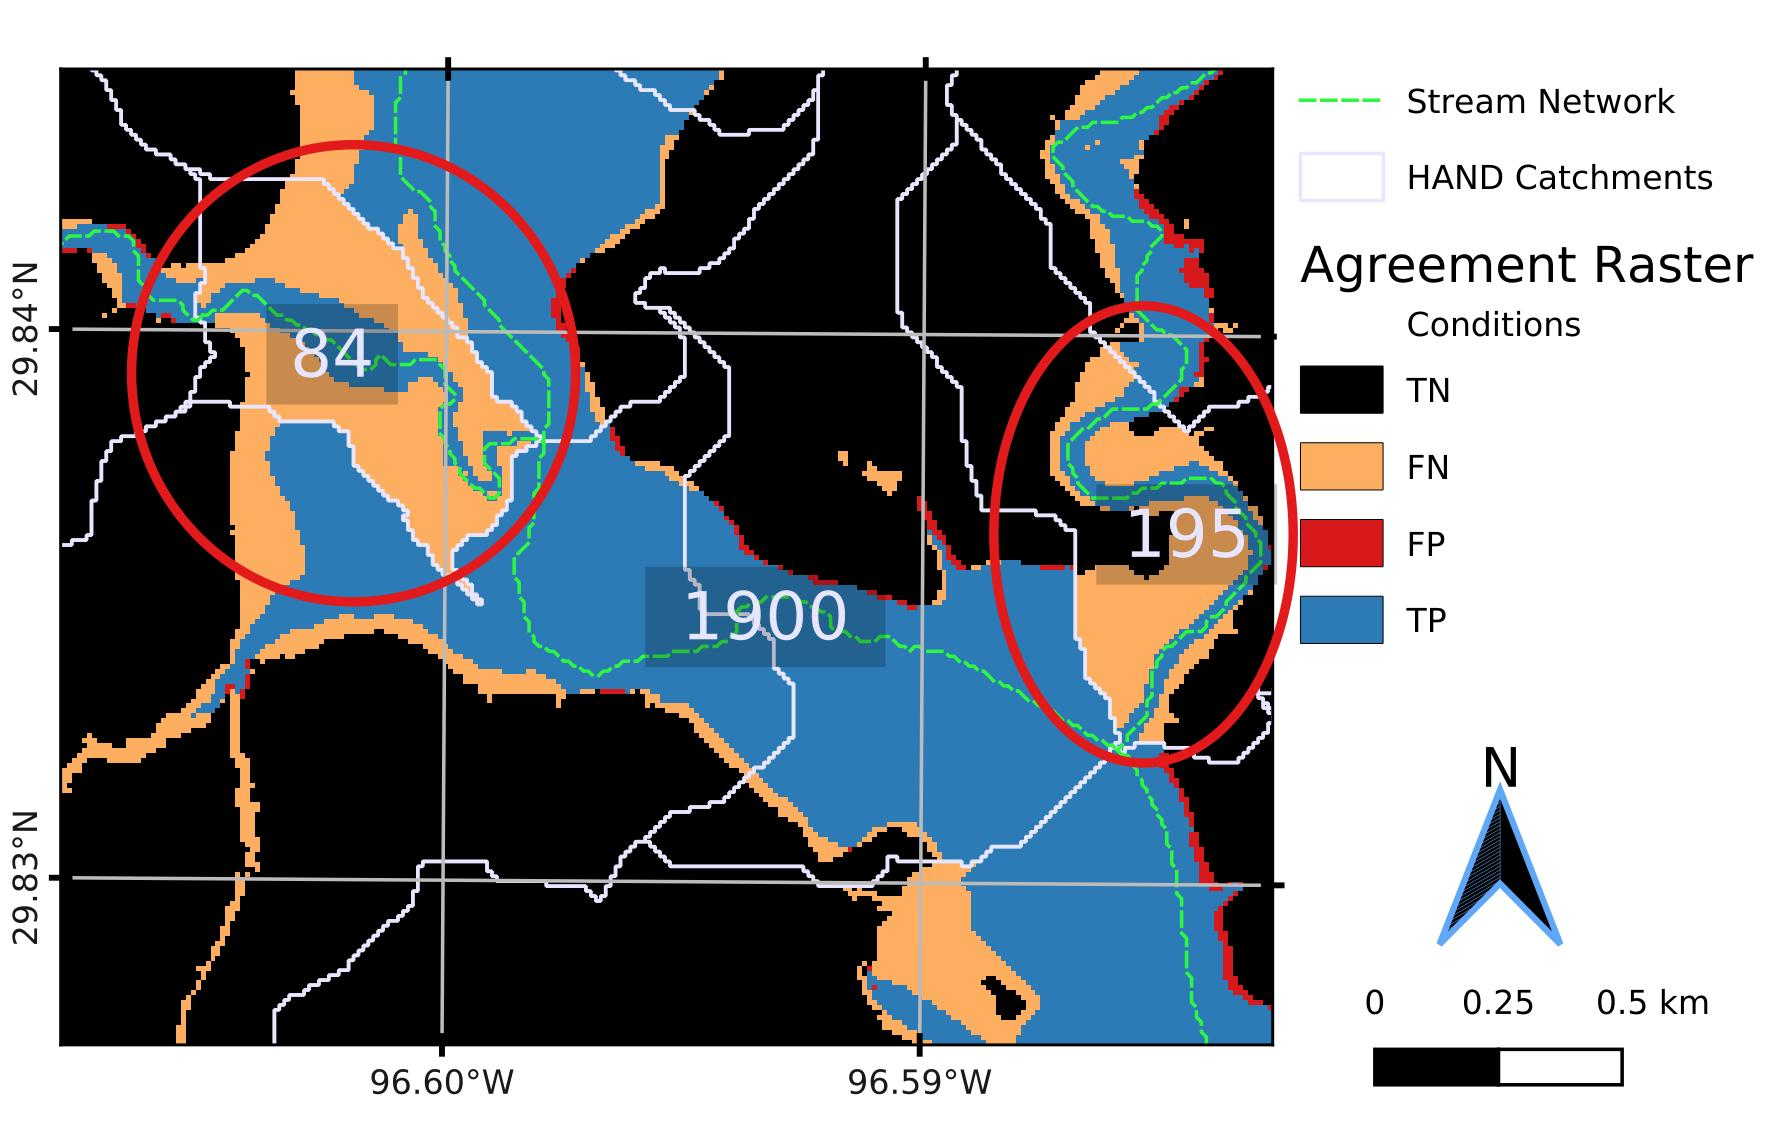
\includegraphics[scale=1.0]{figures/catchment_boundaries_issue.jpg}
\caption{False negatives associated with confluence of tributaries with MS. Integers represent flow values from BLE 100 year event for the associated areas. 
No backwater consideration is implemented and the independent nature of the HAND catchments prohibits pluvial inundation from taking place.}
\label{fig:catchment_boundaries_issue}
\end{figure}
%
We seek to resolve this problem by deriving HAND for processing units with stream networks of reduced stream order. 
We present two successive methods implemented that reduce drainage densities by reducing Horton-Strahler stream orders of the networks employed and test our presented hypothesis that unary stream order networks enhance FIM performance skill with HAND.
The resulting FIMs from the overlapping HAND processing units are mosaiced together taking any inundated area to be inundated but more will be explained in Section \ref{ssec:inundation_mapping}.
%
%%%%%%%%%%%%%%%%%%%%%%%%%%%%%%%%%%%%%%%%%%%%%%%%%%%%%%%%
\subsubsection{NWS Main-stems}
\label{sssec:nws_mainstems}
%
The Mainstems (MS) network is a subset of the NWM full-resolution (FR) network at and downstream of AHPS forecast points as seen in Figure \ref{fig:forecast_points}.
The MS network comprises about 200 thousand km of stream length which is less than 4\% of the FR total stream length of 5.5 million km.
It also spans 121,724 reaches across 1,608 HUC8s.
HAND was originally derived for this stream network to enhance mapping skill along these critical MS segments \cite{djokic2019arc}. 
The inundation derived from this stream network is mosaiced with the inundation from the FR network to form the MS FIMs. 
Within each HUC, you'll typically only find a MS stream network of stream order 1 (i.e. headwater) but this can vary if more than one AHPS forecasting point is found within or upstream of the HUC in question.
%
%%%%%%%%%%%%%%%%%%%%%%%%%%%%%%%%%%%%%%%%%%%%%%%%%%%%%%%%
\subsubsection{Generalized Mainstems}
\label{sssec:generalized_mainstems}
%
To further the efforts implemented by MS, we sought to derive HAND at a level path scale which we call GMS.
Since the MS network only covers a small percentage of the NWM forecasting domain, we sought to expand the benefits of stream order reduction within HAND processing units to the entire FR domain.
Level paths group flowlines by maximizing the length of each flow path and minimizing the number of level path identifiers within a given domain \cite{moore2019user,mckay2012nhdplus}. 
Starting at the outlet, a unique level path is propagated upstream. 
At every confluence, the direction of maximum flow path length is sought to propagate the current level path identifier.
For the remaining parent reaches of the given junction, a new level path identifier is assigned and the process recursively continues with them.
Figure \ref{fig:level_path_methods} illustrate how level paths (symbolized by unique colors) are propagated upstream by the value of arbolate sum.
Each HUC8 is discretized into level paths independently and relevant inputs are assigned to each level path processing unit given a buffer of 7 km.
At the level path scale, the methods in Sections \ref{ssec:hydro_conditioning} and \ref{ssec:deriving_fim_hydrofabric} are executed leaving out any tributaries of the level path in question at the time.
The only exception to this is the use of the NWM stream network directly for use with hydro-enforcement which was motivated by the difficulty in deriving level paths in the NWM stream network with high agreement with the NHDPlusHR stream lines.

To illustrate the GMS procedure, we reference Figure \ref{fig:gms_methods} to show how deriving HAND and FIMs from GMS works.
In Figure \ref{fig:gms_methods}a, we uniquely color code the level paths derived for the NWM stream network. 
For each one of these lines, we derive HAND and its associated datasets including catchments, crosswalks, and rating curves.
Each level path is buffered to a polygon with a user-available distance parameter of 7 km and this polygon is used to subset the original DEM for two selected level paths in Figure \ref{fig:gms_methods}b.
We illustrate two HAND grids for two of the level paths in this HUC8 in Figure \ref{fig:gms_methods}c.
Once the FIM hydrofabrics for each level path are generated, we can inundate them individually also shown in Figure \ref{fig:gms_methods}d.
Lastly these individual FIMs are mosaiced together as explained in Section \ref{ssec:inundation_mapping} and shown in Figure \ref{fig:gms_methods}c.
%
\begin{figure}[h!]
\centering
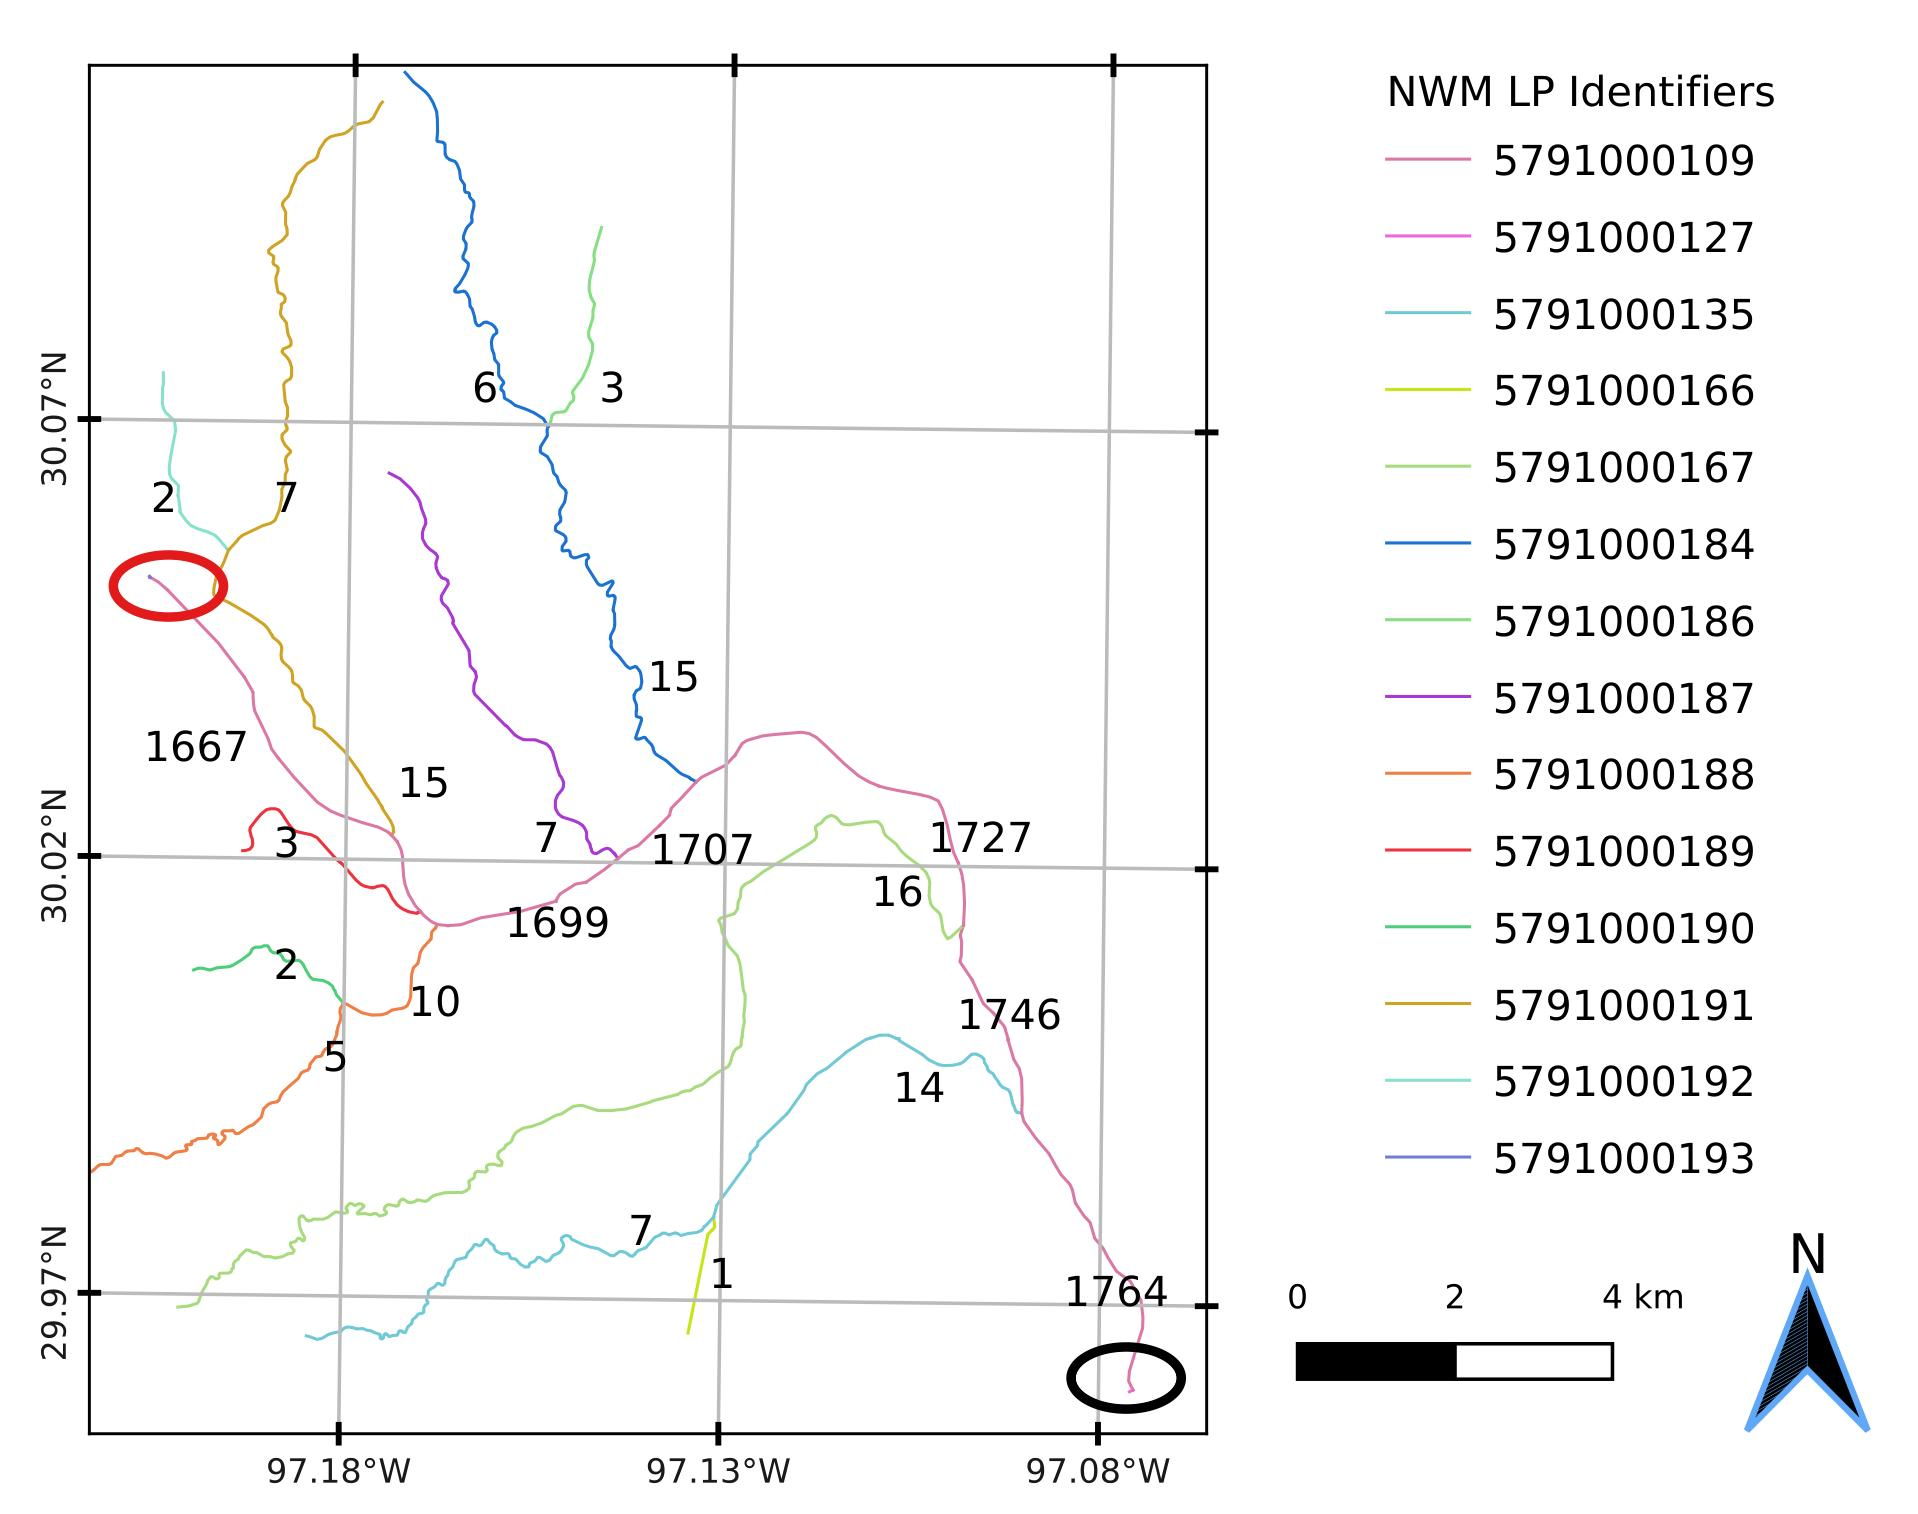
\includegraphics[scale=1.0]{figures/level_path_methods.jpg}
\caption{Illustrates how level paths for the NWM are derived.
Level paths symbolized by lines of unique colors are propagated upstream following the direction of maximum arbolate sum at each junction.
}
\label{fig:level_path_methods}
\end{figure}
%
%
\begin{figure}[h!]
\centering
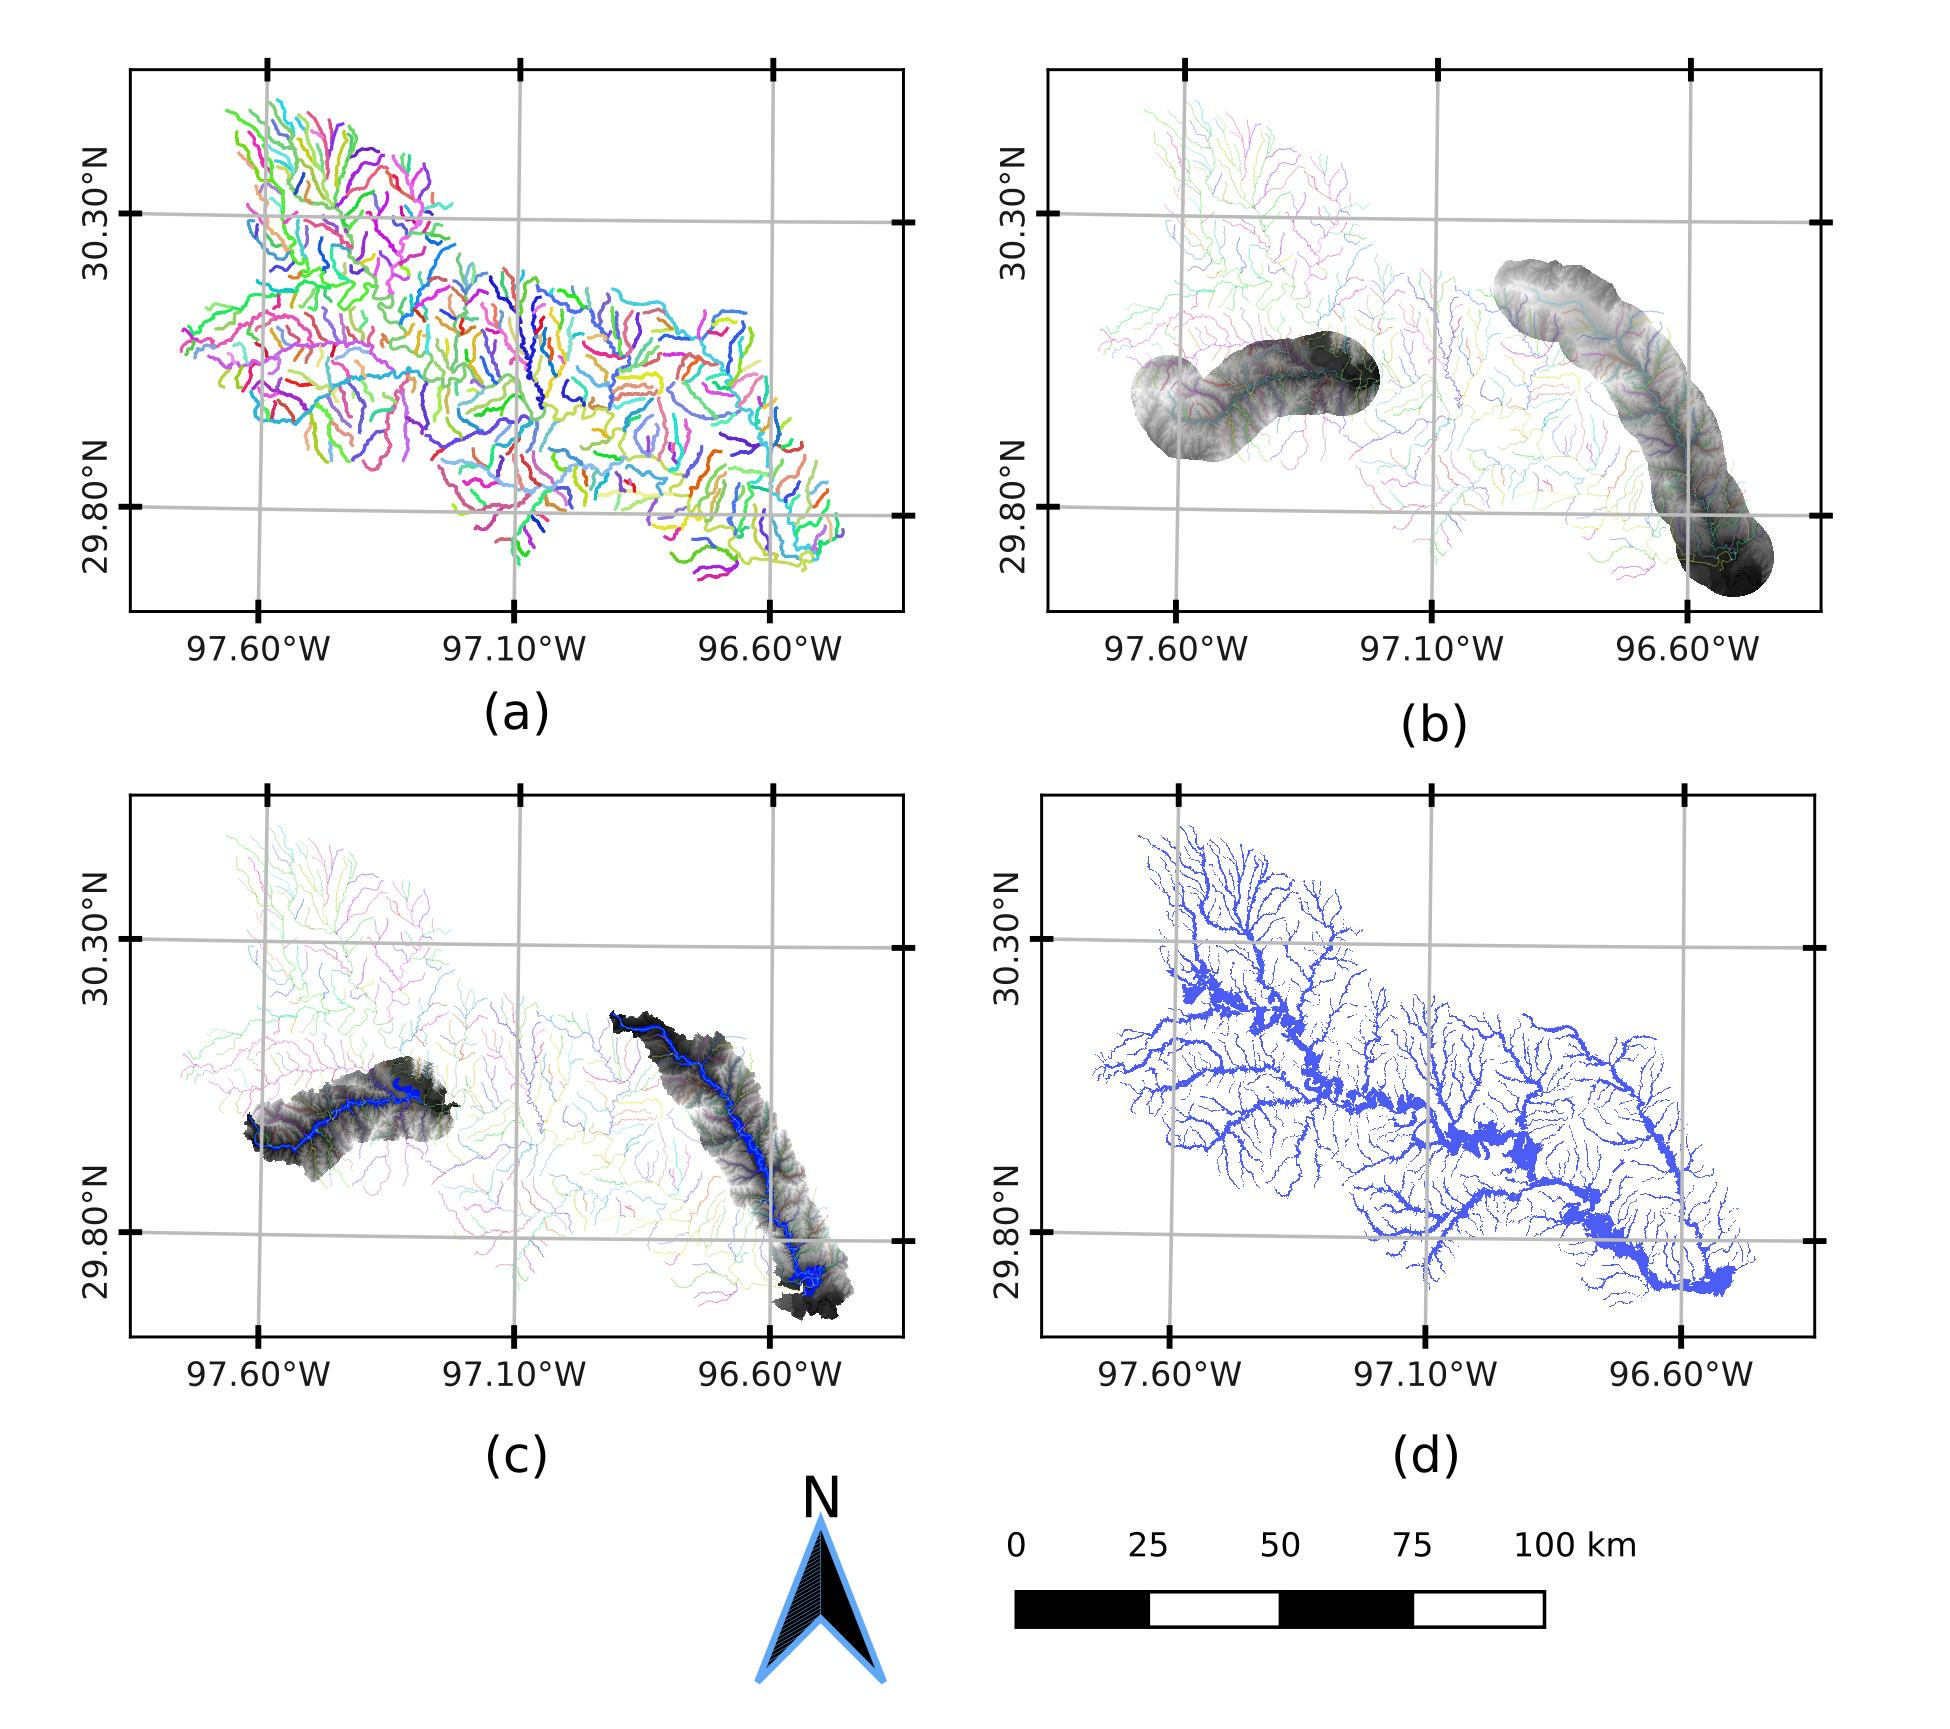
\includegraphics[scale=1.0]{figures/gms_methods.jpg}
\caption{Overall procedure for GMS HAND.
In (a), we illustrate all NWM stream lines symbolized by their level path.
Meanwhile (b), demonstrates the DEM clipped to a 7 km buffer around two selected level paths.
In (c), we show how HAND can be computed just for each one of these two level paths independently. 
We also show inundation maps created for these two level paths in (c). 
In (d), we show all the inundation maps for all the level paths mosaiced together. }
\label{fig:gms_methods}
\end{figure}
%
%%%%%%%%%%%%%%%%%%%%%%%%%%%%%%%%%%%%%%%%%%%%%%%%%%%%%%%%
\subsection{Inundation Mapping}
\label{ssec:inundation_mapping}
%
The FIM hydrofabric consisting of the relative elevations grid, catchments grid, catchment polygons, rating curve, and cross-walking data are all used to convert forecasts from the NWM into forecasts extents.
For operational situations, one would cache the FIM hydrofabric then either produce libraries of FIM for a sample of discharges or stages or also produce the FIM in near real-time (NRT).
From the cached FIM hydrofabric and design or forecast discharges including those extracted from the NWM, inundation maps can be generated at HUC 8 spatial processing units in a rapid, parallel operation. 
The discharges are associated with NWM reach identifiers and cross-walked over to reach identifiers in the FIM hydrofabric.


Utilizing the stage-discharge relationships in the synthetic rating curves, each forecast for each catchment identifier is assigned a stage value. 
The catchments grid encoded with the reach identifiers are used to map the stages by thresholding to the forecast stage.
We use the basic logic already established in previous works to conduct this \cite{nobre2016hand,liu2016cybergis,maidment2017conceptual}.
Mathematically, the HAND values, $H_{ij}$, can be indexed by the reach identifiers, i, and pixel indices, j.
For each forecast stage, $S_i$, one can express the formula for $D_{ij}$, a continuous variable denoting water depth at a given pixel with reach and pixel identifiers i and j respectively in Equation \ref{eq:hand_fim_depth}.
For each forecast stage, $S_i$, one can express the formula for $F_{ij}$, a binary variable denoting inundation condition in Equation \ref{eq:hand_fim} in terms of $D_{ij}$ by simply thresholding at zero depths.
%
\begin{linenomath*}
\begin{equation}
\label{eq:hand_fim_depth}
    D_{ij} = S_i - H_{ij}
\end{equation}
\end{linenomath*}
%
\begin{linenomath*}
\begin{equation}
\label{eq:hand_fim}
    F_{ij} = D_{ij} > 0
\end{equation}
\end{linenomath*}
%
For the cases of MS and GMS, the inundation maps produced for the respective processing units at lower maximum stream orders must be mosaiced together to form a seamless forecast in the form of a single raster file.
For mosaicing the depths, we select the maximum inundation depth from the all the contributing areas K index by its lower case character, k.
Equation \ref{eq:comp_fim_depths} illustrates how the maximum depth from all the contributing areas, k, to each pixel j in catchment i.
Equation \ref{eq:comp_fim} illustrates the same process but for mosaicing the binary inundation maps.
%
\begin{linenomath*}
\begin{equation}
\label{eq:comp_fim_depths}
    D_{ij} = \max_{k=[1,...,K]} D_{ijk}
\end{equation}
\end{linenomath*}
%
For the MS and GMS methods, the contributing areas are defined differently.
For MS, the FIM from MS HAND and FR HAND are mosaiced together to form a singular inundation map thus K is set to 2 for that case.
For GMS, all FIMs from all the level paths in a given area are mosaiced together then K is set to this number of level paths.
Figures \ref{fig:gms_methods}a and \ref{fig:gms_methods}b, illustrate how inundation maps are created for lower stream order processing units then mosaiced together.
%
\begin{linenomath*}
\begin{equation}
\label{eq:comp_fim}
    F_{ij} = \max_{k=[1,...,K]} F_{ijk}
\end{equation}
\end{linenomath*}
%
%%%%%%%%%%%%%%%%%%%%%%%%%%%%%%%%%%%%%%%%%%%%%%%%%%%%%%%%
\subsection{Evaluation}
\label{ssec:evaluation}
%%%%%%%%%%%%%%%%%%%%%%%%%%%%%%%%%%%%%%%%%%%%%%%%%%%%%%%%
%
Evaluation of our relative elevation CFIM method is conducted by comparison to the HEC-RAS 1D derived models produced within FEMA region 6 \cite{fema2021base,fema2021estimated}.
49 HUC 8's spanning about 185 thousand square km were available at the time (now more) across nine states and shown in Figure \ref{fig:all_ble_maps}.
The maps to the 1\% recurrence flow (1 in 100 year) and the 0.2\% recurrence flow (1 in 500 year) are furnished by InFRM so we used those corresponding discharges and mapping extents for evaluation.
We did exclude NWM V2.1 Reservoirs from evaluation because these are not properly accounted for in the inundation.
By using the same HEC-RAS derived discharges and FIM extents, we are able to separate out errors introduced by hydrology, atmospheric forcings, hydraulic routing, etc that we would have potentially seen if we used NWM forecasted discharges.
Figure \ref{fig:ble_evaluation_method} illustrates both NWM V2.1 and BLE stream lines as well as the BLE cross-sections that have recurrence discharges associated with them.
We elected to spatially intersect the HEC-RAS cross sections with the NWM stream network assigning the 1\% and 0.2\% flow rates to each NWM reach. 
To handle multiple intersections, we opted to use a filter to select the median discharge value attributed to each NWM reach.
This partially handles the influence of neighboring cross sections that could cause flow discontinuities and mass conservation issues.
Additionally, the stream network of the InFRM furnished models are of higher stream densities and bifurcation ratios, as evident in Figure \ref{fig:ble_evaluation_method}, leading to a significant amount of false negatives (FN) (under-prediction) along headwater streams with Horton-Strahler orders of one due to the lack of representation of these additional headwater streams in the NWM network.
While the limitations are noted, this method does best to detangle the influence of exogenous variables that we do not wish to study in this comparison.
%
\begin{figure}[h!]
\centering
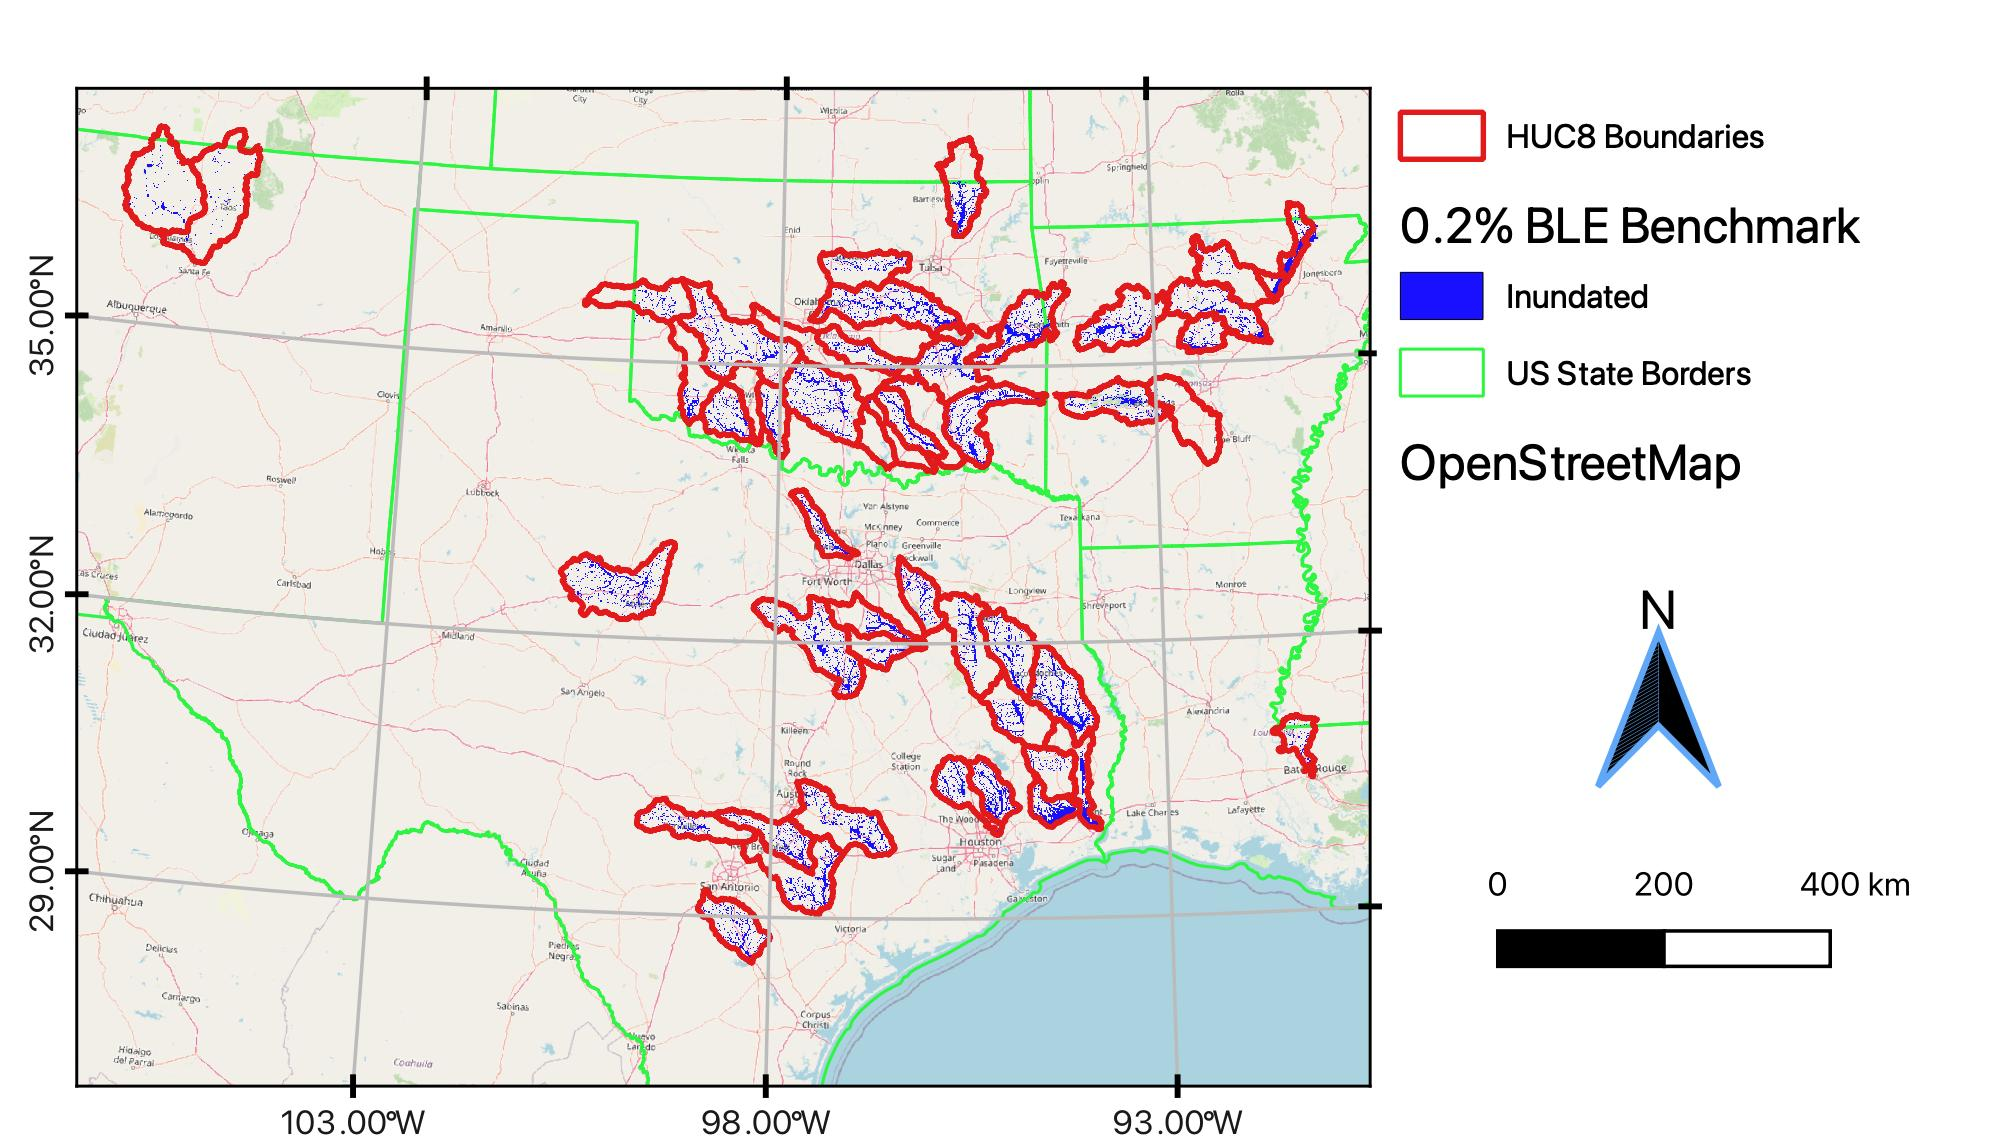
\includegraphics[scale=1.0]{figures/all_ble_maps.jpg}
\caption{Shows 185 thousand square km of modeled areas for BLE domain of 49 HUC8s across 9 states. This dataset for 1\% and 0.2\% recurrence flows were used as benchmarks.}
\label{fig:all_ble_maps}
\end{figure}
%
\begin{figure}[h!]
\centering
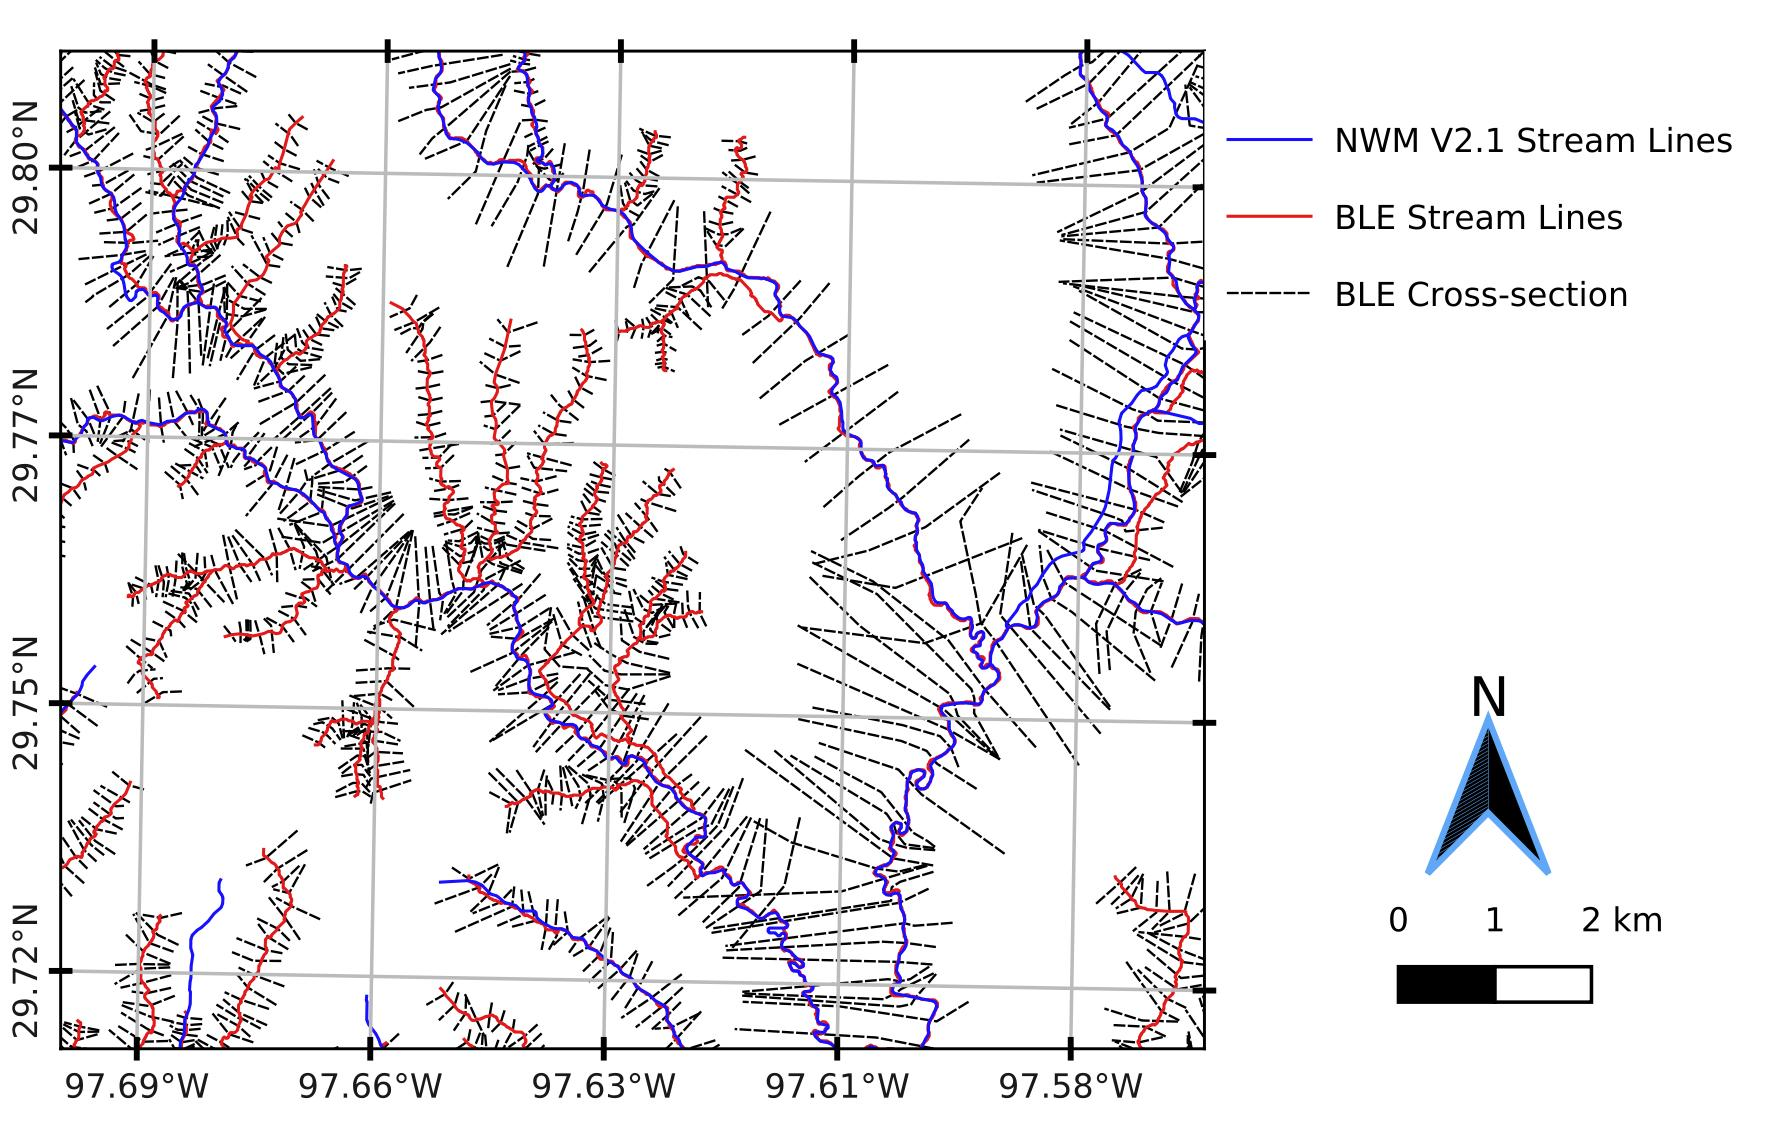
\includegraphics[scale=1.0]{figures/ble_evaluation_method.jpg}
\caption{Illustrates Base Level Engineering (BLE) cross sections and stream lines. The BLE stream network, which is denser than the NWM V2.1 stream lines, is also shown. BLE cross sections are intersected with NWM reaches and the median recurrence discharge for 1\% and 0.2\% levels are selected per NWM reach. }
\label{fig:ble_evaluation_method}
\end{figure}
%
The metrics employed in this study to evaluate inundation extents include Critical Success Index (CSI), Probability of Detection (POD), and False Alarm Ratio (FAR) and presented in Equations \ref{eq:csi}, \ref{eq:pod}, \ref{eq:far}, respectively.
To calculate these secondary metrics, one must define three primary metrics including true positives (TP) which is predicted wet and wet in benchmark dataset.
The two types of errors consist of false positives (FP), or type I errors, which is dry in benchmark but predicted wet and false negatives (FN), or type II errors, which is wet in benchmark by predicted dry. 
Lastly, the reader may come across true negatives (TN) which is defined as dry in both the benchmark and predicted datasets.
Maximizing POD indicates a model's ability to detect the given threat of interest, inundation, while minimizing FAR is sought to indicate a models ability in reducing FN errors.
Some work by \citeA{gerapetritis2004behavior} while at the NWM denotes CSI a good proxy for measuring a forecasting system's utility in protecting life and property and has been shown to be optimized mathematically when $POD = 1 - FAR$.
While these metrics are commonly employed in the evaluation of FIM and binary weather prediction communities in general, they do come with some notable limitations including frequency dependence in the case of CSI and FAR \cite{gerapetritis2004behavior,stephens2014problems,schaefer1990critical,jolliffe2012forecast}.
Thus, frequency dependent statistics should be used with caution when comparing across sites with varying frequencies. 
Lastly, approximately 6 HUC8s do not have NWM MS reaches thus we imputed the metrics for FR for these sites as the best available forecasting capability.
%
\begin{linenomath*}
\begin{equation}
\label{eq:csi}
CSI = \frac{TP}{TP + FN + FP}
\end{equation}
\end{linenomath*}
%
\begin{linenomath*}
\begin{equation}
\label{eq:pod}
POD = \frac{TP}{TP + FN}
\end{equation}
\end{linenomath*}
%
\begin{linenomath*}
\begin{equation}
\label{eq:far}
FAR = \frac{FP}{TP + FP}
\end{equation}
\end{linenomath*}
%
 %
% Results
\clearpage % this clears figures before references
%%%%%%%%%%%%%%%%%%%%%%%%%%%%%%%%%%%%%%%%%%%%%%%%%%%%%%%%
%%%%%%%%%%%%%%%%%%%%%%%%%%%%%%%%%%%%%%%%%%%%%%%%%%%%%%%%
\section{Results}
\label{sec:results}
%%%%%%%%%%%%%%%%%%%%%%%%%%%%%%%%%%%%%%%%%%%%%%%%%%%%%%%%
%%%%%%%%%%%%%%%%%%%%%%%%%%%%%%%%%%%%%%%%%%%%%%%%%%%%%%%%
%
%%%%%%%%%%%%%%%%%%%%%%%%%%%%%%%%%%%%%%%%%%%%%%%%%%%%%%%%
\subsection{Mapping Performance}
\label{ssec:mapping_performance}
%%%%%%%%%%%%%%%%%%%%%%%%%%%%%%%%%%%%%%%%%%%%%%%%%%%%%%%%
%
We produced FIMs for the entire BLE domain within the 49 HUC8 areas across several states in the south central US. 
The forecasted FIMs using the discharges for the 1\% (100 year) and 0.2\% (500 year) recurrence flows directly from HEC-RAS were used to avoid noise and errors from hydrological processes.
We computed the statistics (CSI, POD, and FAR) for both 100 and 500 year events for Mannings N set to 0.06 and 0.12. 
The distribution of these statistics can be examined in Figure \ref{fig:violin_plot} as violin plots.
Each half of a violin plot represents the kernel density estimation (KDE) for a given model (FR, MS, GMS), given Manning's n value (0.06, 0.12), and given recurrence interval (1\%, 0.2\%), and performance metric (CSI, POD, FAR).
We also denote trend lines for each metric and Manning's n setting as well as their respective slope estimate and one-tailed p-value denoting the level of significance of the trend.

Aggregating the metrics in the method above treats each HUC8 as it's own unit and does little to consider the size differences of the HUCs. 
In an opposing aggregation method, we illustrate in Table \ref{tab:aggregate_metrics}  the CSI, POD, and FAR recomputed for the entire domain using the sum of all the TPs, FPs, and FNs. 
%
\begin{figure}[h!]
\centering
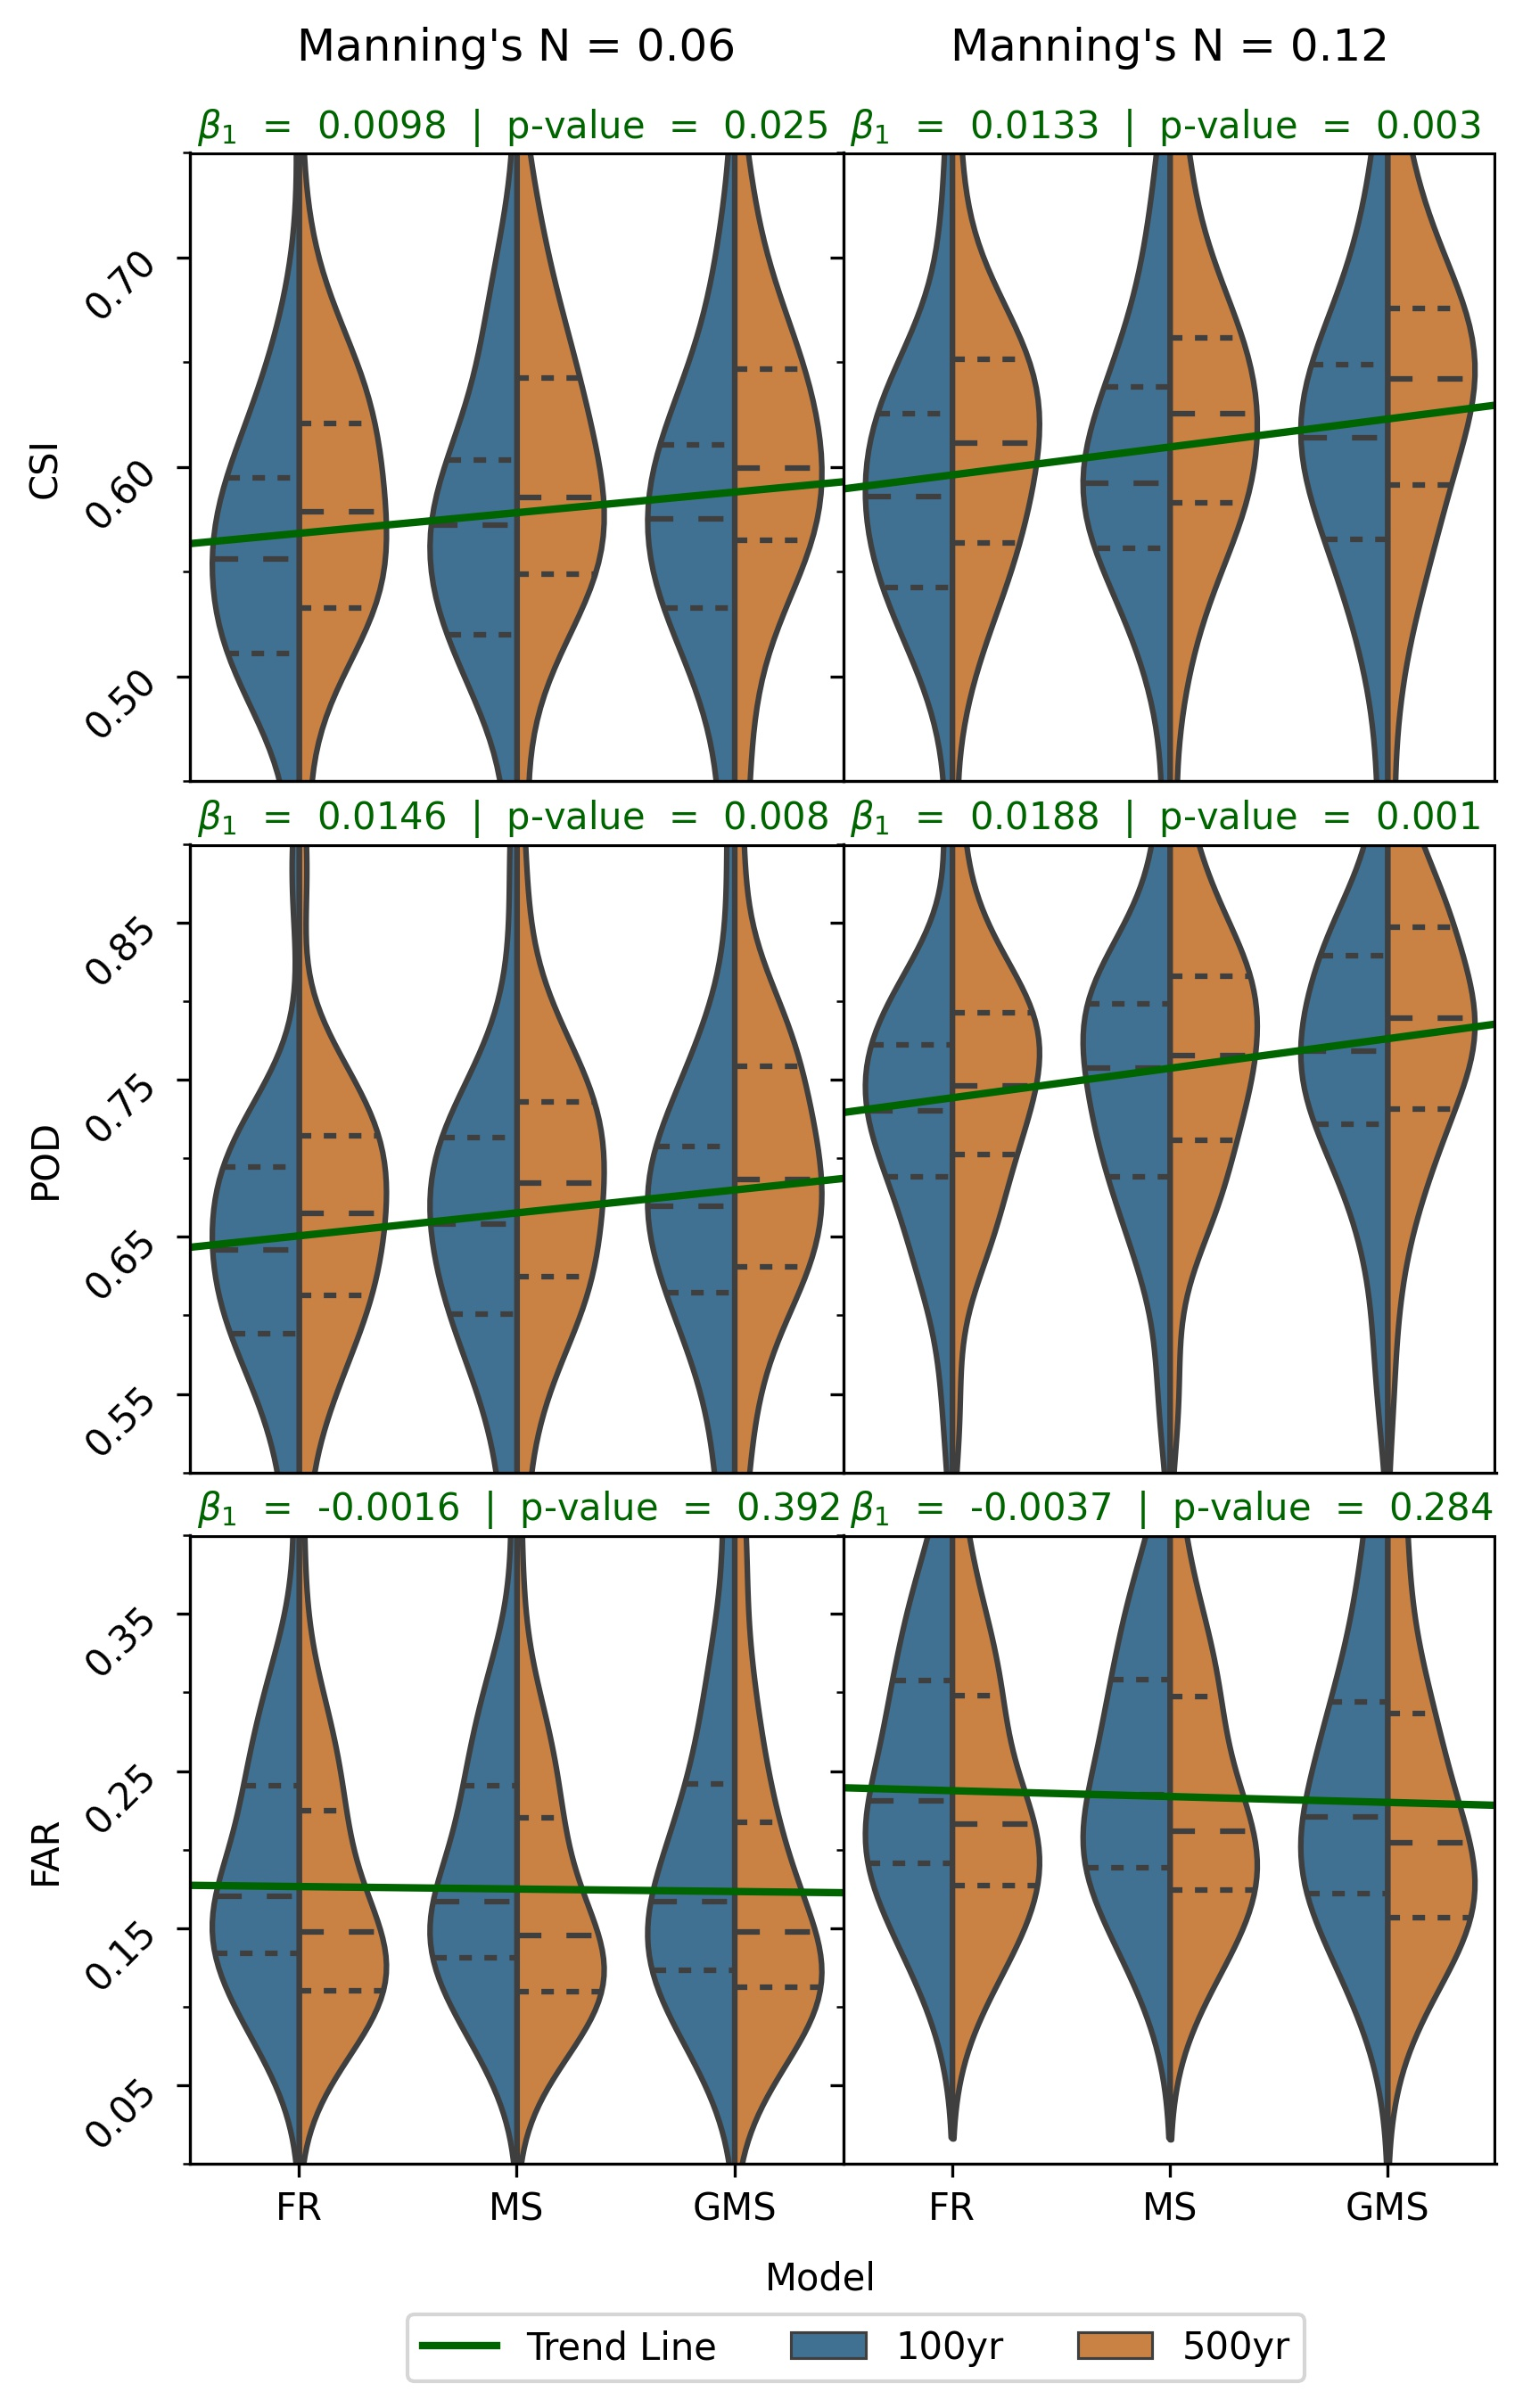
\includegraphics[scale=0.9]{figures/violin_plots.jpg}
\caption{Shows kernel density estimation of the distributions (sample size = 49) for 1\% (100 year) and 0.2\% (500 year) along with horizontal, dashed lines for the 25th, 50th, and 75th percentiles (in order from bottom to top).
The sub-figures separate the combination of three metrics (CSI, POD, and FAR) for two settings of Manning's n (0.06 and 0.12).
Trend lines for each metric - Mannings combination are shown (sample size = 294) along with associated slope and p-value of slope testing one-tailed significance.}
\label{fig:violin_plot}
\end{figure}
%
\begin{table}[h!]
\caption{Recomputed CSI, POD, and FAR using the primary metrics, TPs, FPs, and FNs, aggregated for BLE domain.
         The best value across models is highlighted in bold.}
\label{tab:aggregate_metrics}
\centering
%\begin{tabular}{|p{2cm}|p{2cm}|p{2cm}|p{2cm}|}
\begin{tabular}{|c|c||c|c|c|c|c|c|}
\hline
\multirow{2}{*}{Metric} & \multirow{2}{*}{Manning's n} & \multicolumn{2}{|c|}{FR} & \multicolumn{2}{|c|}{MS} & \multicolumn{2}{|c|}{GMS} \\
\cline{3-8}
  &  & 100yr & 500yr & 100yr & 500yr & 100yr & 500yr \\
\hline
\multirow{2}{*}{CSI} & 0.06 & 0.5576 & 0.5839 & 0.5717 & 0.5990 & \textbf{0.5796} & \textbf{0.6075} \\
\cline{2-8}
  & 0.12 & 0.5915 & 0.6149 & 0.6054 & 0.6288 & \textbf{0.6182} & \textbf{0.6435} \\
\hline
\multirow{2}{*}{POD} & 0.06 & 0.6354 & 0.6575 & 0.6524 & 0.6755 & \textbf{0.6633} & \textbf{0.6863} \\
\cline{2-8}
  & 0.12 & 0.7255 & 0.7446 & 0.7460 & 0.7648 & \textbf{0.7606} & \textbf{0.7810} \\
\hline
\multirow{2}{*}{FAR} & 0.06 & 0.1800 & 0.1609 & 0.1787 & \textbf{0.1589} & \textbf{0.1778} & \textbf{0.1589} \\
\cline{2-8}
  & 0.12 & 0.2379 & 0.2208 & 0.2374 & 0.2204 & \textbf{0.2324} & \textbf{0.2148} \\
\hline
\end{tabular}
\end{table}
%
% Interpretation of metrics
From Figure \ref{fig:violin_plot} and Table \ref{tab:aggregate_metrics}, we denote several meaningful trends. 
Using CSI as an overall proxy for skill of the FIM, we note that generally speaking the skill is correlated with a reduction of the stream orders of the processing units used for HAND.
In other words, the more we derive HAND on networks of unit drainage density and mosaic the resulting FIMs, the better those FIMs perform.
While this trend is evident for both sets of Manning's n values, the trend is slightly more significant for the higher value of 0.12.
Other trends related to this Figure include the general performance premium for 0.2\% events as opposed to lower 1\% events.
We also note how the higher Manning's n value enhances performance for both of these recurrence intervals across all models.

Dissecting the improvements and trends presented in the previous paragraph comes down mostly to improvement in POD or a reduction in absolute amount of FNs.
POD being the primary driver in skill enhancement is evident across models by comparing the slope of the POD lines with the slope of the FAR lines.
Even though aggregating metrics by HUC8 yields a statistically zero trend, one does see a slight reduction in FAR across models that reduce HAND's maximum stream order.
Additionally, we note that POD is a primary driver in enhancing performance across Manning's n values as well.
This significant improvement comes at a cost of false alarms as the FAR increases significantly across Manning's n values.
%
%%%%%%%%%%%%%%%%%%%%%%%%%%%%%%%%%%%%%%%%%%%%%%%%%%%%%%%%
\subsection{Computational Performance}
\label{ssec:compuational_performance}
%%%%%%%%%%%%%%%%%%%%%%%%%%%%%%%%%%%%%%%%%%%%%%%%%%%%%%%%
%
The NFIE experiments were able to produce HAND for 331 HUC6's in 1.34 CPU years \cite{liu2016cybergis} and estimates using work from \citeA{djokic2019arc} put producing HAND at the FR NWM at 0.55 CPU years. 
For our work, we were able to produce HAND at the full NWM resolution in 0.13 CPU years which represents a substantial speed-up compared to previous works.
For the MS resolution an additional, 0.05 CPU years is required on top of this bringing the total to about 0.18 CPU years to produce 2,188 HUC8s that span additional areas not covered in previous HAND versions including Hawaii and Puerto Rico.
GMS which generalizes HAND production to level path scale adds a significant amount of CPU time to the process bringing the estimate total to about 1.17 CPU years.
%
 %
% Discussion
\clearpage % this clears figures before references
%%%%%%%%%%%%%%%%%%%%%%%%%%%%%%%%%%%%%%%%%%%%%%%%%%%%%%%%
%%%%%%%%%%%%%%%%%%%%%%%%%%%%%%%%%%%%%%%%%%%%%%%%%%%%%%%%
\section{Discussion}
\label{sec:discussion}
%%%%%%%%%%%%%%%%%%%%%%%%%%%%%%%%%%%%%%%%%%%%%%%%%%%%%%%%
%%%%%%%%%%%%%%%%%%%%%%%%%%%%%%%%%%%%%%%%%%%%%%%%%%%%%%%%
%
Overall, we note a positive relationship between FIM skill and a reduction of the stream order of the stream network we use to derive the HAND datasets.
Most of this change is accounted for by increasing POD thus reducing FNs especially along higher order rivers with higher flow magnitudes.
We note that reducing stream order does in turn suffer from diminishing returns in which the increase in mapping skill for applying stream order reduction to roughly 4-5\% of the stream network is about the same as the increase for applying stream order reduction to the remaining 95-96\% of the stream network.
This motivates further work in identifying what the optimal coverage of stream order reduction could be and how to parameterize that coverage. 
One option could be removing stream orders ones and possibly twos and threes from stream order reduction and simply using the inundation from FR from these areas.

In analyzing the data, we found a slight reduction in FAR was detected and more digging pointed to a bias in rating curves introduced by stream order reduction.
Figure \ref{fig:rating_curve_comparison} illustrates the general effect that stream order reduction has on synthetic rating curves.
Sub-figure \ref{fig:rating_curve_comparison}a shows how the average rating curves for all reaches for stage values 0 to 25 meters at one-third meter intervals tend to bias down (and to the right) with ever increasing stream order reduction (FR to MS to GMS). 
This bias is more pronounced for GMS since that implements stream order reduction down to the unit level for the entire FR network while MS only does so for 4-5\% of the network.
Attempting to diagnose this bias in the SRC leads one to Equation \ref{eq:reach_averaged_mannings_equation} which shows the reach averaged synthetic rating curve relationship between stage and discharge.
Across the three methods explored, FR, MS, and GMS, one identifies differences in the inputs and outputs and notes no difference in the stages and Manning's n values.
While the channel slope and reach lengths are not exactly the same across methods, their averaged differences are very negligible which only leaves room for deviations in volume and bed area.
Again, volume (V(y) or simply V) is synonymous to reach-averaged cross-sectional area and bed area (B(y) or B) is analogous to reach-averaged hydraulic radius.
Discharge, Q, is directly related to volume and inversely related to bed area and each parameter is weighed according to the magnitude of its exponent which are $\frac{5}{3}$ and $\frac{2}{3}$ respectively (see Equation \ref{eq:reach_averaged_mannings_equation}). 
Figures \ref{fig:rating_curve_comparison} b and c show how volume and bed area compare across the three methods with GMS having significantly greater values than MS which has greater values than FR.
Again the relative discrepancy between FR vs MS and MS vs GMS is explained by the extent of their spatial coverages.
Both V and B values increase but are weighed differently by their respective exponents and pull Q in different directions.
We show in Figure \ref{fig:rating_curve_comparison}d the relationship of $\frac{V^{5/3}}{B^{2/3}}$ and plot this ratio against stage, y, to show how these two parameters collectively pull the rating curve Q up and biases the rating curve down.
In other words, the magnitude and weight of the volume at each stage level exceeds the influence of the magnitude and weight of the bed area.
Both parameters are set to increase mainly due to much larger catchments leading to more pixels at each stage level as shown in Figure \ref{fig:rating_curve_comparison}e.
Much of the increase in inundated pixels, volume, and bed area can be explained by much larger catchments that encompass neighboring tributaries.
These tributaries have a significant amount of bathymetry that is low-lying thus easily including the SRC derivation. 
They also contribute volume and bed area that is technically not perpendicular to the flux of streamflow being accounted for in the stream in question. 
Careful examination of Figure \ref{fig:gms_enhancement}b shows how much larger catchments include neighboring tributaries and the geometry associated with those tributaries. 
This geometry is not perpendicular to the flow that is associated with the main reach thus leading to biases in the SRC.
We consider this fact to have a nuanced effect on skill, while reducing the rate of FPs it also can lead to FNs due to biases in the SRC.

Additional careful analysis of Figure \ref{fig:gms_enhancement}a, leads one to note many catchments that don't have inundation or significant inundation.
While the cause of these errors can be varied, we assert here that conflating 4 networks for use in evaluations leads to significant error.
As one may remember, Section \ref{sssec:cross_walking_networks} details how reach identifiers are conflated for the FIM network back to that of the NWM. 
One of the issues is when a reach of given stream order accidentally conflates to that of a neighboring tributary that is of lower order which leads to areas of FNs.
The utilization of MS and GMS only conflates to NWM catchments directly associated with the level path in question which is inherently easy to do with those methods. 
Thus part of the improvement in MS and GMS methods is due to a slight improvement in cross-walking methodology.
The NWM stream network was derived using the NHD medium resolution dataset which was derived from coarser DEMs than those used here. 
Additional conflation is identified in cross-walking the stream network used by the BLE maps and those of HAND.
Until a singular stream network is used for the NWM, BLE benchmark, and for HAND based FIM, conflation will continue being a source of error.

Our qualitative analysis suggests that the synthetic rating curves offer a significant opportunity for improvement in HAND based FIM for future development.
The bathymetry of the 10 m DEM from 3DEP is known to be lacking proper representation thus leading to inadequate representation of volume and bed area with all three methods employed.
Manning's n which typically accounts for roughness could be tuned to account for these DEM limitations or could be held fixed to some local value associated with a given flood magnitude.
Some adjusting parameter must be introduced to enhance the estimation of the bathymetric representation.
Lidar DEMs from the USGS at 3 m and 1 m scale could be utilized to derive HAND as well which we conject should show better agreement with higher fidelity FIMs also derived from the same Lidar based DEMs.

Lastly, after errors introduced by conflation, poor roughness estimation, bathymetric/elevation adjustment are accounted for, HAND still has another fundamental limitation that is inherently baked into how it works.
For HAND to be derived and thus create a FIM for a given area, that area must entirely drain to the stream network and the stream network must also drain itself.
In other words, an entire area eligible for flooding must monotonically decrease in elevation. 
DEM's naturally don't do this and the dynamics of true flood events don't follow drainage patterns.
Enforcing this assumption for HAND leads to significant amount of DEM manipulations that introduce basic errors.
These errors are deep into the assumptions of HAND and thus more difficult to disentangle.
Ultimately, the use of more advanced 2-D hydrodynamic models should be considered for dealing with this limitation of HAND but would come at significant expense at the given high resolution across very large spatial scales and frequent forecast resolutions.
%
\begin{figure}[h!]
\centering
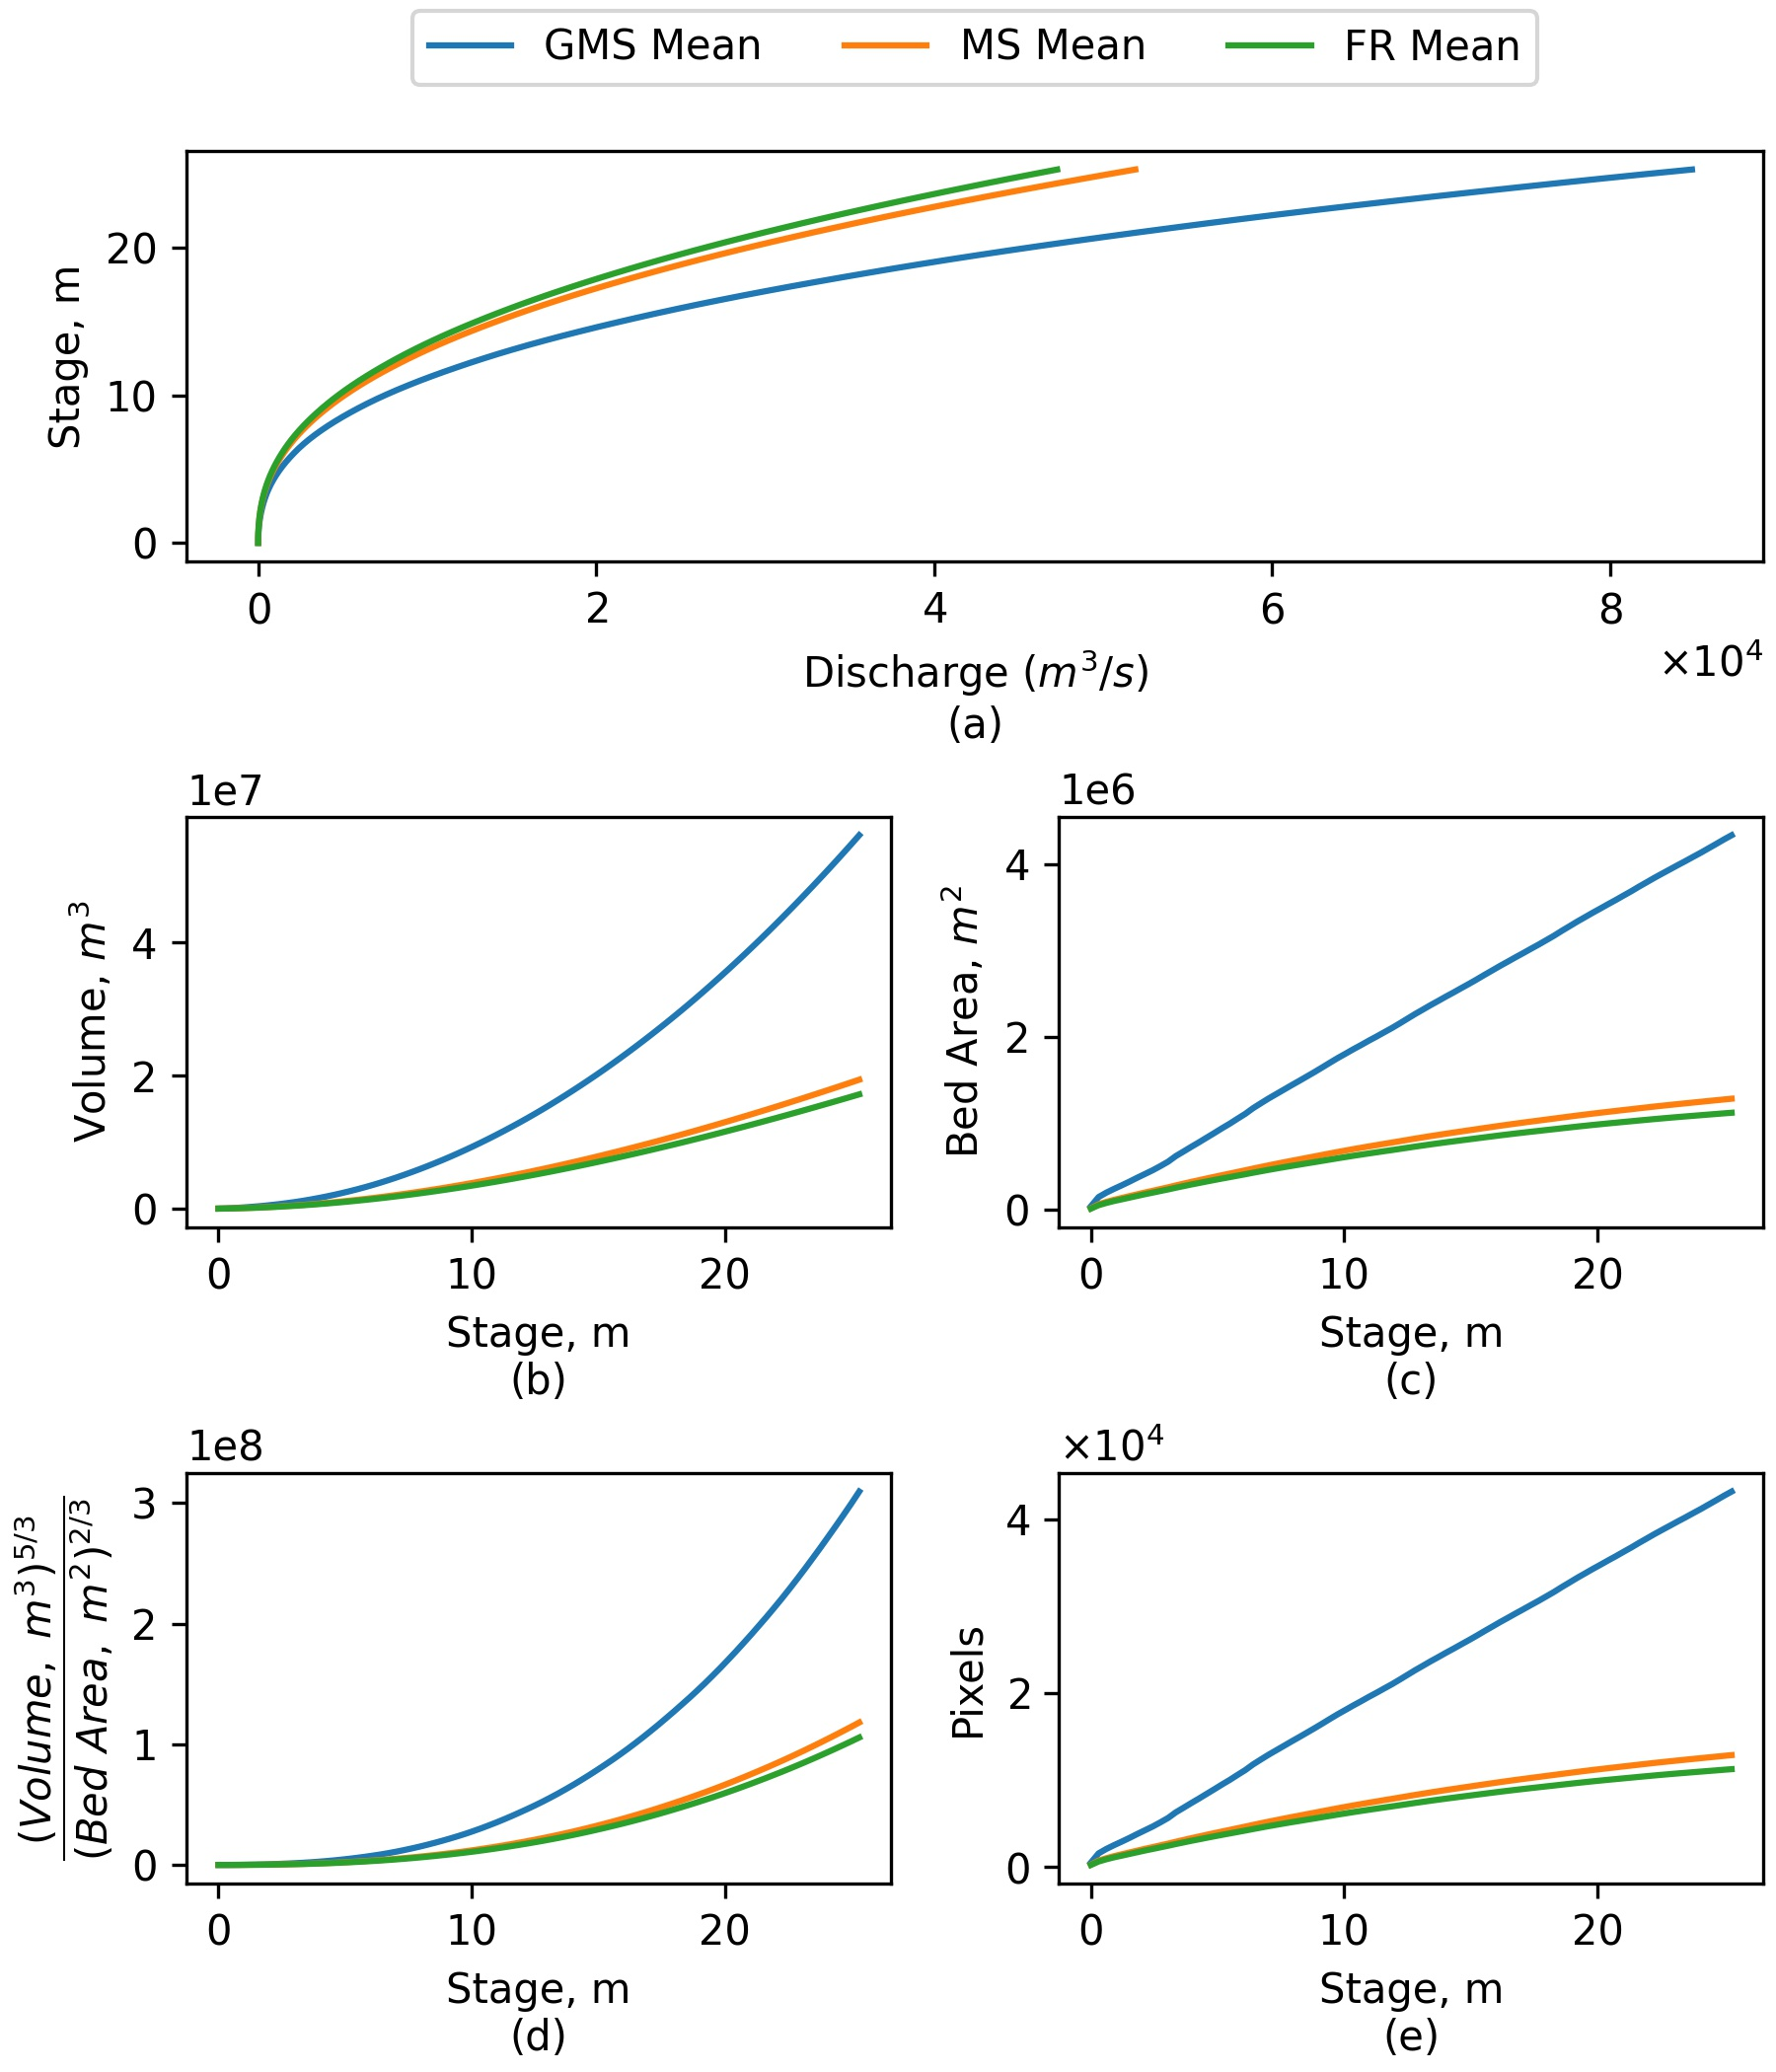
\includegraphics[scale=1.0]{figures/rating_curve_comparison.jpg}
\caption{Illustrates average quantities for the three methods, FR, MS, and GMS, for each stage value (m). 
The values are (a) Discharge $m^3s^{-1}$, (b) Volume $m^3$, (c) Bed Area $m^2$, (d) a function of Volume and Bed Area, and (e) number of pixels.
}
\label{fig:rating_curve_comparison}
\end{figure}
%
%
\begin{figure}[h!]
\centering
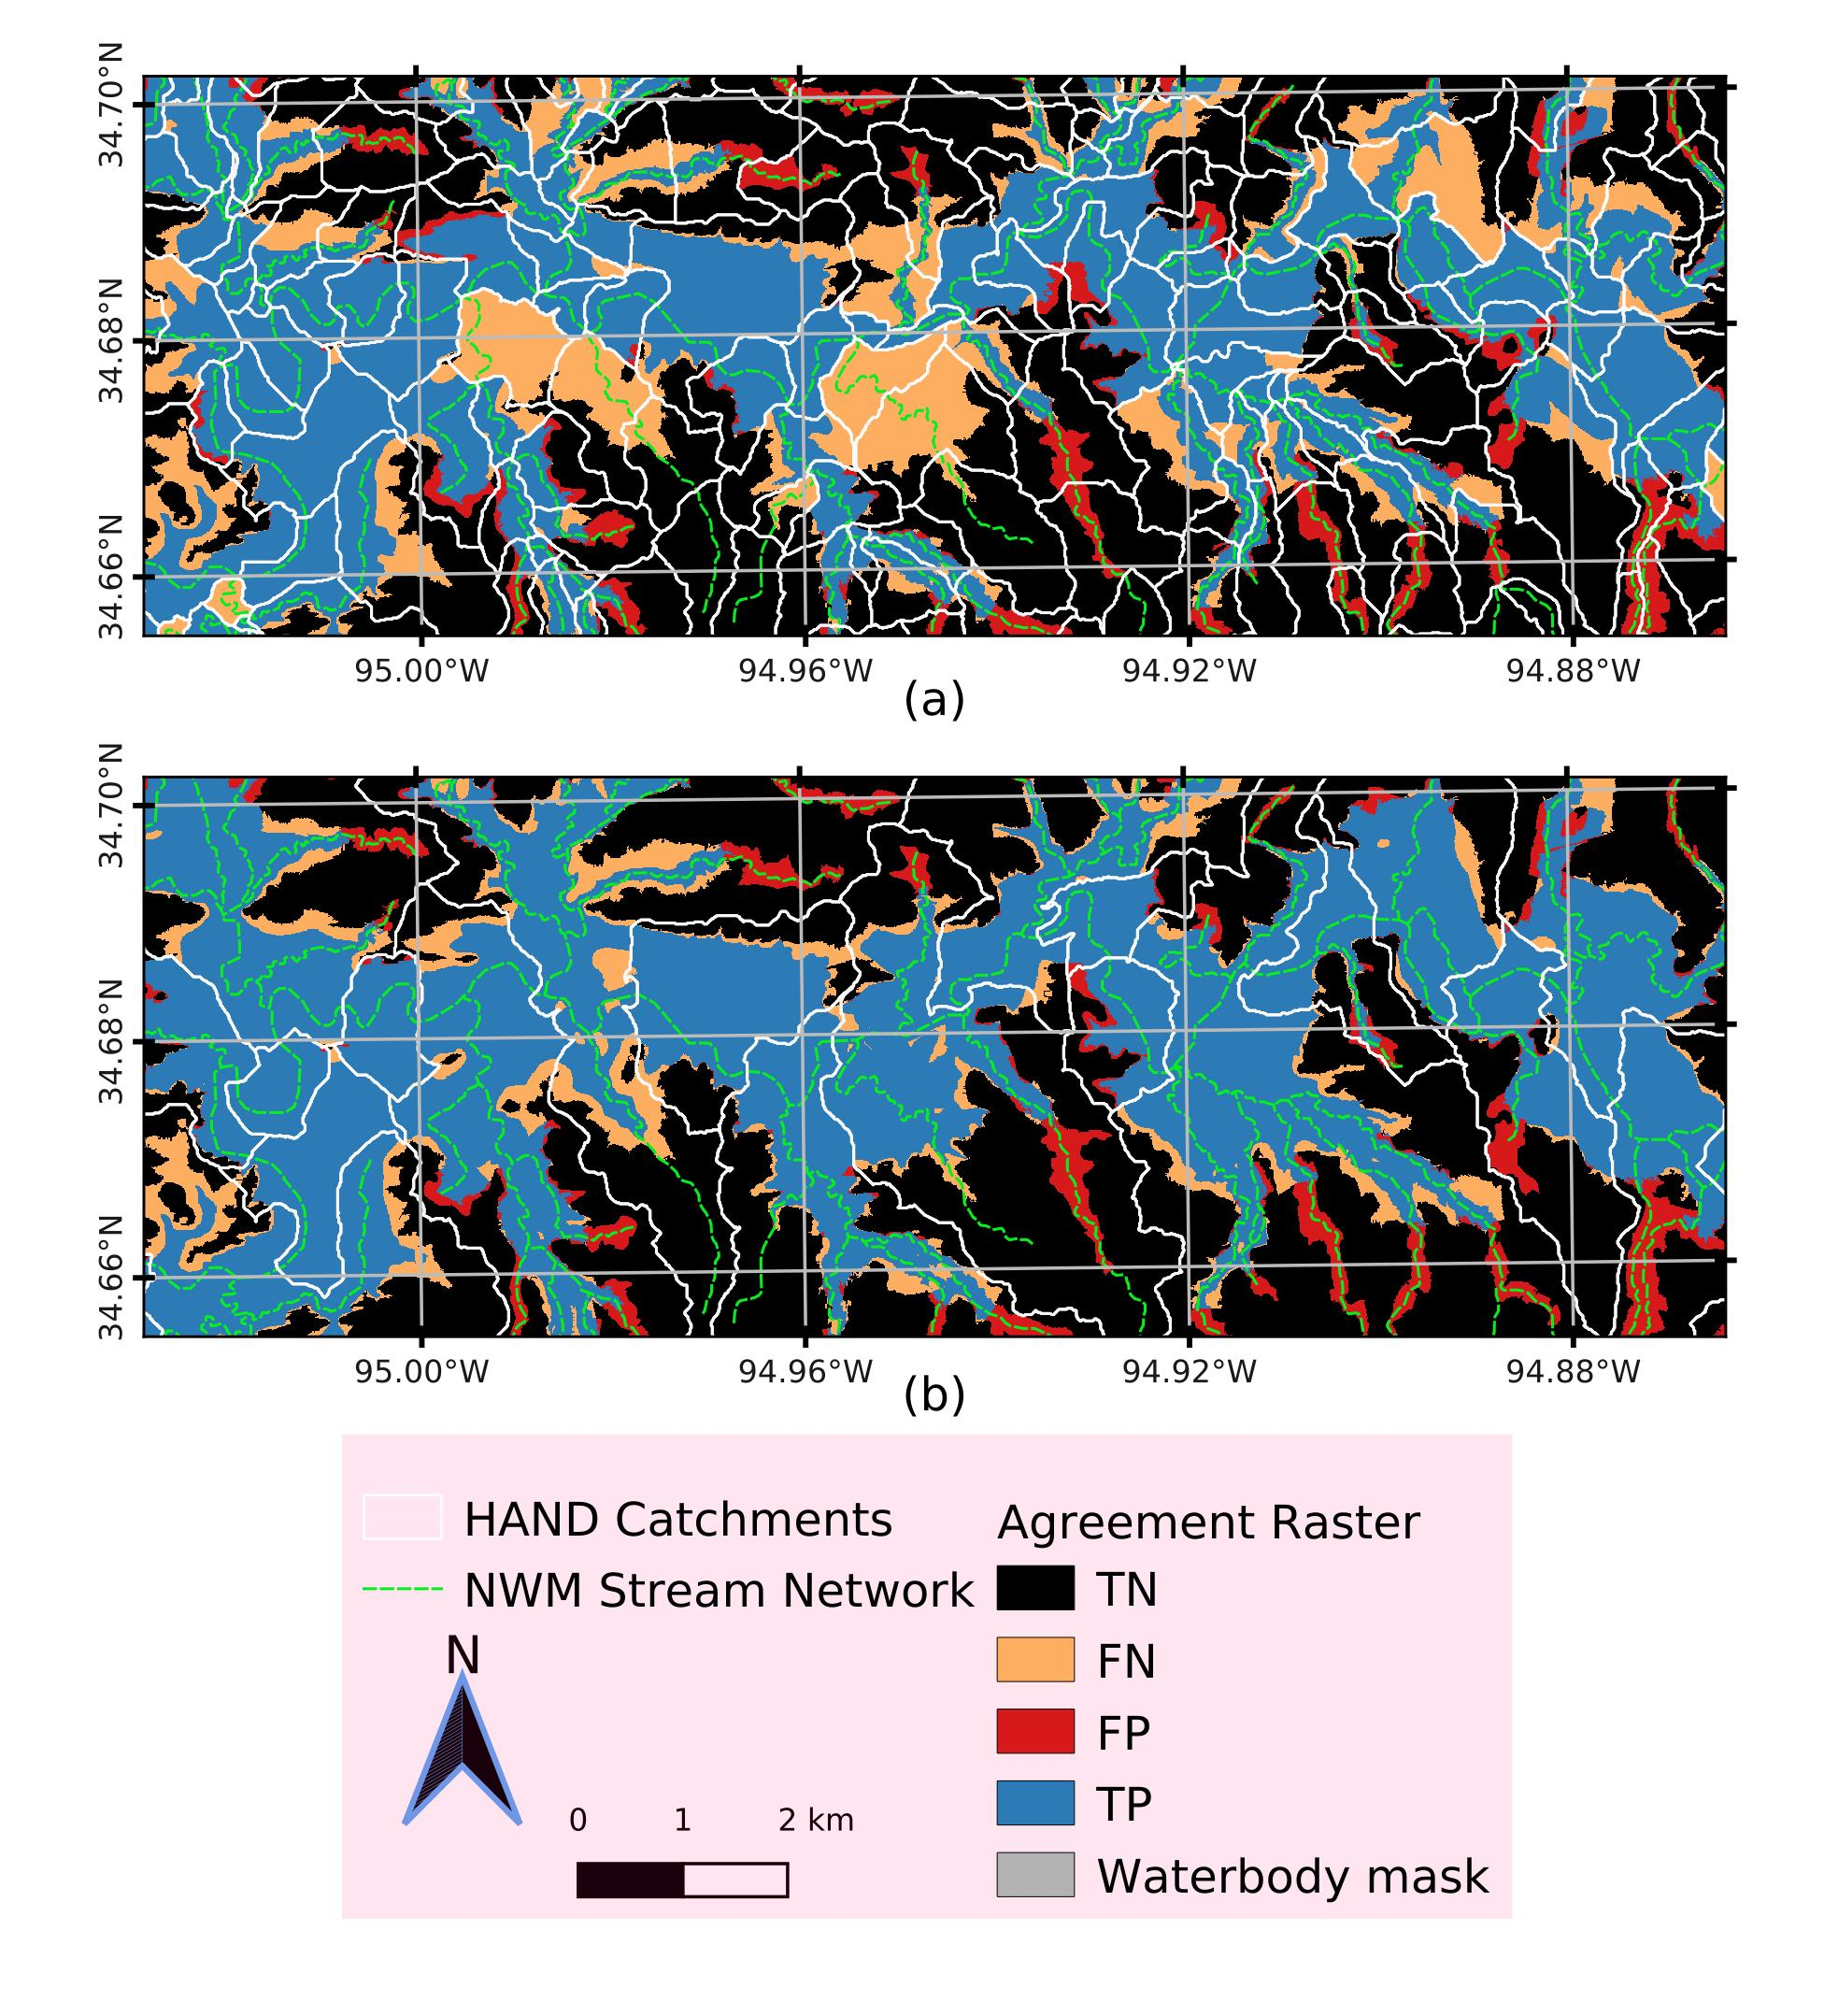
\includegraphics[scale=1.0]{figures/gms_enhancement.jpg}
\caption{OWP FIM inundation agreement, TP, FP, FN, and TN, with BLE HEC-RAS maps in HUC 11140105.
Catchment boundaries and stream lines are shown in white and dotted green, respectively.
Sub-figure (a) shows agreement of FR HAND denoting significant areas of under-prediction due to junctions and catchment boundaries.
Meanwhile, (b) shows the agreement for GMS and much larger catchments leading to much better inundation agreement for this given reach. 
Overall, this illustrates the benefits of stream order reduction for deriving HAND datasets.
}
\label{fig:gms_enhancement}
\end{figure}
%
 %
% Conclusions
\clearpage % this clears figures before references
%%%%%%%%%%%%%%%%%%%%%%%%%%%%%%%%%%%%%%%%%%%%%%%%%%%%%%%%
%%%%%%%%%%%%%%%%%%%%%%%%%%%%%%%%%%%%%%%%%%%%%%%%%%%%%%%%
\section{Conclusions}
\label{sec:conclusions}
%%%%%%%%%%%%%%%%%%%%%%%%%%%%%%%%%%%%%%%%%%%%%%%%%%%%%%%%
%%%%%%%%%%%%%%%%%%%%%%%%%%%%%%%%%%%%%%%%%%%%%%%%%%%%%%%%
%
Floods present a significant, under-served, and expanding risk to life, property, and resources.
Previous flood forecasting systems lacked the coverage to adequately inform society of these risks.
The National Water Model (NWM) developed by the National Oceanic and Atmospheric Administration's Office of Water Prediction, along with partners, provides increased spatial coverage and resolution as well as additional forecast time horizons on mostly hourly intervals.
Additional processing is required to convert streamflows from the NWM to river stages and finally to flood inundation maps (FIM).
Height Above Nearest Drainage (HAND) is a means of detrending digital elevations maps (DEM) by normalizing elevation to the nearest relevant drainage point.
HAND coupled with the use of reach averaged synthetic rating curves (SRC) provide such a means of creating continental scale FIM capabilities at high resolutions (1/3 arc-second, 10 m) and high temporal frequencies (up to 1 hr).
Scalable, open-source software was developed to produce HAND and associated datasets (catchments, SRCs, and cross-walking data) for the NWM forecasting area including Hawaii and Puerto Rico \cite{inundationMapping2022}.
HAND is produced using the latest hydro-conditioning techniques to enforce monotonically decreasing elevations including stream burning, levee enforcement, pit-filling, stream channel excavation, thalweg breaching, headwater seeding, stream reach resampling, and more. 
Finally, we use this implementation to investigate the skill of the FIMs by varying the scale of the processing units used to derive HAND.
We illustrate that reducing the Horton-Strahler stream order of a HAND processing unit down to one enhances skill by significantly reducing false negatives at junctions of major streams.
This also affects the parameters used to compute stage-discharge relationships biasing discharge higher at given stages which reduced the rate of false positives.
FIM skill was evaluated over large spatial scales by comparison to HEC-RAS 1D models.
Further investment in the SRC's is warranted by accounting for bathymetric errors inherited by the DEM and better accounting for localized friction values at varying flow magnitudes.
Utilizing the highest resolution Lidar and bathymetric data should also improve the vertical accuracy of HAND and better account for fine grain features that greatly affect inundation extents.
Due to inherent limitations with HAND, scalable, physics-based methods are necessary to consider to provide a better representation of flood extent dynamics in steady and unsteady conditions. 
%
 %
%%

%  Numbered lines in equations:
%  To add line numbers to lines in equations,
%  \begin{linenomath*}
%  \begin{equation}
%  \end{equation}
%  \end{linenomath*}


%% Enter Figures and Tables near as possible to where they are first mentioned:
%
% DO NOT USE \psfrag or \subfigure commands.
%
% Figure captions go below the figure.
%\section{= enter section title =}
%Text here ===>>>
%\section{= enter section title =}
%Text here ===>>>
%%

%  Numbered lines in equations:
%  To add line numbers to lines in equations,
%  \begin{linenomath*}
%  \begin{equation}
%  \end{equation}
%  \end{linenomath*}



%% Enter Figures and Tables near as possible to where they are first mentioned:
%
% DO NOT USE \psfrag or \subfigure commands.
%
% Figure captions go below the figure.
% Table titles go above tables;  other caption information
%  should be placed in last line of the table, using
% \multicolumn2l{$^a$ This is a table note.}
%
%----------------
% EXAMPLE FIGURES
%
% \begin{figure}
% \includegraphics{example.png}
% \caption{caption}
% \end{figure}
%
% Giving latex a width will help it to scale the figure properly. A simple trick is to use \textwidth. Try this if large figures run off the side of the page.
% \begin{figure}
% \noindent\includegraphics[width=\textwidth]{anothersample.png}
%\caption{caption}
%\label{pngfiguresample}
%\end{figure}
%
%
% If you get an error about an unknown bounding box, try specifying the width and height of the figure with the natwidth and natheight options. This is common when trying to add a PDF figure without pdflatex.
% \begin{figure}
% \noindent\includegraphics[natwidth=800px,natheight=600px]{samplefigure.pdf}
%\caption{caption}
%\label{pdffiguresample}
%\end{figure}
%
%
% PDFLatex does not seem to be able to process EPS figures. You may want to try the epstopdf package.
%

%
% ---------------
% EXAMPLE TABLE
%
% \begin{table}
% \caption{Time of the Transition Between Phase 1 and Phase 2$^{a}$}
% \centering
% \begin{tabular}{l c}
% \hline
%  Run  & Time (min)  \\
% \hline
%   $l1$  & 260   \\
%   $l2$  & 300   \\
%   $l3$  & 340   \\
%   $h1$  & 270   \\
%   $h2$  & 250   \\
%   $h3$  & 380   \\
%   $r1$  & 370   \\
%   $r2$  & 390   \\
% \hline
% \multicolumn{2}{l}{$^{a}$Footnote text here.}
% \end{tabular}
% \end{table}

%% SIDEWAYS FIGURE and TABLE
% AGU prefers the use of {sidewaystable} over {landscapetable} as it causes fewer problems.
%
% \begin{sidewaysfigure}
% \includegraphics[width=20pc]{figsamp}
% \caption{caption here}
% \label{newfig}
% \end{sidewaysfigure}
%
%  \begin{sidewaystable}
%  \caption{Caption here}
% \label{tab:signif_gap_clos}
%  \begin{tabular}{ccc}
% one&two&three\\
% four&five&six
%  \end{tabular}
%  \end{sidewaystable}

%% If using numbered lines, please surround equations with \begin{linenomath*}...\end{linenomath*}
%\begin{linenomath*}
%\begin{equation}
%y|{f} \sim g(m, \sigma),
%\end{equation}
%\end{linenomath*}

%%% End of body of article

%%%%%%%%%%%%%%%%%%%%%%%%%%%%%%%%
%% Optional Appendix goes here
%
% The \appendix command resets counters and redefines section heads
%
% After typing \appendix
%
%\section{Here Is Appendix Title}
% will show
% A: Here Is Appendix Title
%
%\appendix
%\section{Here is a sample appendix}

%%%%%%%%%%%%%%%%%%%%%%%%%%%%%%%%%%%%%%%%%%%%%%%%%%%%%%%%%%%%%%%%
%
% Optional Glossary, Notation or Acronym section goes here:
%
%%%%%%%%%%%%%%
% Glossary is only allowed in Reviews of Geophysics
%  \begin{glossary}
%  \term{Term}
%   Term Definition here
%  \term{Term}
%   Term Definition here
%  \term{Term}
%   Term Definition here
%  \end{glossary}

%
%%%%%%%%%%%%%%
% Acronyms
%   \begin{acronyms}
%   \acro{Acronym}
%   Definition here
%   \acro{EMOS}
%   Ensemble model output statistics
%   \acro{ECMWF}
%   Centre for Medium-Range Weather Forecasts
%   \end{acronyms}

%
%%%%%%%%%%%%%%
% Notation
%   \begin{notation}
%   \notation{$a+b$} Notation Definition here
%   \notation{$e=mc^2$}
%   Equation in German-born physicist Albert Einstein's theory of special
%  relativity that showed that the increased relativistic mass ($m$) of a
%  body comes from the energy of motion of the body—that is, its kinetic
%  energy ($E$)—divided by the speed of light squared ($c^2$).
%   \end{notation}




%%%%%%%%%%%%%%%%%%%%%%%%%%%%%%%%%%%%%%%%%%%%%%%%%%%%%%%%%%%%%%%%
%
%  ACKNOWLEDGMENTS
%
% The acknowledgments must list:
%
% >>>>	A statement that indicates to the reader where the data
% 	supporting the conclusions can be obtained (for example, in the
% 	references, tables, supporting information, and other databases).
%
% 	All funding sources related to this work from all authors
%
% 	Any real or perceived financial conflicts of interests for any
%	author
%
% 	Other affiliations for any author that may be perceived as
% 	having a conflict of interest with respect to the results of this
% 	paper.
%
%
% It is also the appropriate place to thank colleagues and other contributors.
% AGU does not normally allow dedications.


\acknowledgments
This work was funded by the OWP which is part of NOAA's National Weather Service.
Lynker, under contract with OWP, facilitated this work and computational resources used in research and development.
We would like to thank some notable contributors of this work including Chief Scientist at OWP, Fred Ogden for his technical expertise.
Additionally, David Blodgett from the USGS Water Mission Area was instrumental in helping define level paths and other hydrographic work.
More information on code availability, usage, and data retrieval for OWP FIM is available on GitHub \cite{inundationMapping2022}.
Thanks to the Earth and Space Science Informatics Partnership (ESIP) for storing data from this study for public use and dissemination helping to provide transparent datasets for further collaboration with the research community \cite{esipData2022}.
%The [type of data] data used for [brief context, description] in the study are available at [repository, source name] via [DOI, persistent identifier link] with  [license, access conditions] [optional in-text citation in References]
%[Version number] of the [software name] used for [brief context, description of what the software was used for] is preserved at [DOI, persistent identifier link], available via [license type, access conditions] and developed openly at [software development platform link].* [optional in-text citation in References].


%% ------------------------------------------------------------------------ %%
%% References and Citations

%%%%%%%%%%%%%%%%%%%%%%%%%%%%%%%%%%%%%%%%%%%%%%%
%
% \bibliography{<name of your .bib file>} don't specify the file extension
%
% don't specify bibliography style
%%%%%%%%%%%%%%%%%%%%%%%%%%%%%%%%%%%%%%%%%%%%%%%
%
\clearpage % this clears figures before references
\bibliography{bibliography/owp_fim4_2022}
%
%Reference citation instructions and examples:
%
% Please use ONLY \cite and \citeA for reference citations.
% \cite for parenthetical references
% ...as shown in recent studies (Simpson et al., 2019)
% \citeA for in-text citations
% ...Simpson et al. (2019) have shown...
%
%
%...as shown by \citeA{jskilby}.
%...as shown by \citeA{lewin76}, \citeA{carson86}, \citeA{bartoldy02}, and \citeA{rinaldi03}.
%...has been shown \cite{jskilbye}.
%...has been shown \cite{lewin76,carson86,bartoldy02,rinaldi03}.
%... \cite <i.e.>[]{lewin76,carson86,bartoldy02,rinaldi03}.
%...has been shown by \cite <e.g.,>[and others]{lewin76}.
%
% apacite uses < > for prenotes and [ ] for postnotes
% DO NOT use other cite commands (e.g., \citet, \citep, \citeyear, \nocite, \citealp, etc.).
%



\end{document}



%%%% More Information and Advice:

%% ------------------------------------------------------------------------ %%
%
%  SECTION HEADS
%
%% ------------------------------------------------------------------------ %%

% Capitalize the first letter of each word (except for
% prepositions, conjunctions, and articles that are
% three or fewer letters).

% AGU follows standard outline style; therefore, there cannot be a section 1 without
% a section 2, or a section 2.3.1 without a section 2.3.2.
% Please make sure your section numbers are balanced.
% ---------------
% Level 1 head
%
% Use the \section{} command to identify level 1 heads;
% type the appropriate head wording between the curly
% brackets, as shown below.
%
%An example:
%\section{Level 1 Head: Introduction}
%
% ---------------
% Level 2 head
%
% Use the \subsection{} command to identify level 2 heads.
%An example:
%\subsection{Level 2 Head}
%
% ---------------
% Level 3 head
%
% Use the \subsubsection{} command to identify level 3 heads
%An example:
%\subsubsection{Level 3 Head}
%
%---------------
% Level 4 head
%
% Use the \subsubsubsection{} command to identify level 3 heads
% An example:
%\subsubsubsection{Level 4 Head} An example.
%
%% ------------------------------------------------------------------------ %%
%
%  IN-TEXT LISTS
%
%% ------------------------------------------------------------------------ %%
%
% Do not use bulleted lists; enumerated lists are okay.
% \begin{enumerate}
% \item
% \item
% \item
% \end{enumerate}
%
%% ------------------------------------------------------------------------ %%
%
%  EQUATIONS
%
%% ------------------------------------------------------------------------ %%

% Single-line equations are centered.
% Equation arrays will appear left-aligned.

Math coded inside display math mode \[ ...\]
 will not be numbered, e.g.,:
 \[ x^2=y^2 + z^2\]

 Math coded inside \begin{equation} and \end{equation} will
 be automatically numbered, e.g.,:
 \begin{equation}
 x^2=y^2 + z^2
 \end{equation}


% To create multiline equations, use the
% \begin{eqnarray} and \end{eqnarray} environment
% as demonstrated below.
\begin{eqnarray}
  x_{1} & = & (x - x_{0}) \cos \Theta \nonumber \\
        && + (y - y_{0}) \sin \Theta  \nonumber \\
  y_{1} & = & -(x - x_{0}) \sin \Theta \nonumber \\
        && + (y - y_{0}) \cos \Theta.
\end{eqnarray}

%If you don't want an equation number, use the star form:
%\begin{eqnarray*}...\end{eqnarray*}

% Break each line at a sign of operation
% (+, -, etc.) if possible, with the sign of operation
% on the new line.

% Indent second and subsequent lines to align with
% the first character following the equal sign on the
% first line.

% Use an \hspace{} command to insert horizontal space
% into your equation if necessary. Place an appropriate
% unit of measure between the curly braces, e.g.
% \hspace{1in}; you may have to experiment to achieve
% the correct amount of space.


%% ------------------------------------------------------------------------ %%
%
%  EQUATION NUMBERING: COUNTER
%
%% ------------------------------------------------------------------------ %%

% You may change equation numbering by resetting
% the equation counter or by explicitly numbering
% an equation.

% To explicitly number an equation, type \eqnum{}
% (with the desired number between the brackets)
% after the \begin{equation} or \begin{eqnarray}
% command.  The \eqnum{} command will affect only
% the equation it appears with; LaTeX will number
% any equations appearing later in the manuscript
% according to the equation counter.
%

% If you have a multiline equation that needs only
% one equation number, use a \nonumber command in
% front of the double backslashes (\\) as shown in
% the multiline equation above.

% If you are using line numbers, remember to surround
% equations with \begin{linenomath*}...\end{linenomath*}

%  To add line numbers to lines in equations:
%  \begin{linenomath*}
%  \begin{equation}
%  \end{equation}
%  \end{linenomath*}



